% ---
% title: From Samples to Bits：讲稿与背景知识
% date: 2026-10-02
% tag: Slides
% excerpt: 配合幻灯片 From Samples to Bits 的讲稿。第一部分从傅里叶变换讲起，补齐采样定理、熵与率失真、变换编码、JPEG、小波、学习型压缩和压缩感知等全部背景，让演讲者真正理解要讲的内容；第二部分是逐页要对观众说的话；第三部分是提问准备、公式卡和参考文献。
% ---
\usetikzlibrary{arrows.meta,positioning,calc,decorations.pathreplacing}
\pgfplotsset{compat=1.18}
\definecolor{sig}{HTML}{1F5FAD}
\definecolor{hot}{HTML}{C0392B}
\definecolor{accent}{HTML}{C77C02}
\definecolor{soft}{HTML}{8C8C8C}
\definecolor{video}{HTML}{2E7D6B}
\newcommand{\sinc}{\operatorname{sinc}}

\begin{abstract}
这是幻灯片 \href{https://mejistus.github.io/\#post=Slides/From-Samples-to-Bits.tex}{From Samples to Bits} 的讲稿，分三部分。
\textbf{第一部分（背景知识，第~\ref{sec:fourier}--\ref{sec:link}~节）}是写给演讲者自己的：从傅里叶变换讲起，把采样定理、熵与无损编码、率失真理论、变换编码、JPEG、小波、视频式编码、学习型压缩和压缩感知需要的知识补齐，每个结论都给出推导或直觉，目标是让你不看幻灯片也能把每一页讲清楚、答得出追问。
\textbf{第二部分（逐页讲稿，第~\ref{sec:script}~节）}是要对观众说的话，每页只有要点和一段可以照着说的稿子。
\textbf{第三部分（速查，第~\ref{sec:qa}~节起）}是提问准备、公式卡、术语对照和参考文献。
建议的准备顺序：先通读第一部分（约两小时），再对着幻灯片把第二部分读出声两遍，最后合上讲稿，只看幻灯片讲一遍。
\end{abstract}

\section{这场报告讲什么}\label{sec:overview}

\subsection{一句话主线}
把一个连续信号存成文件，要先\emph{采样}成一串数，再\emph{编码}成比特，所以
\[
\text{比特数}=\text{样本数}\times\text{每个样本的比特数}.
\]
采样定理回答第一个因子：不丢信息最少要多少样本。压缩回答第二个因子：每个样本最少要多少比特。报告的核心论点是：\textbf{这两个因子不是独立的。}比特预算有限时，最优的有损编码本来就会丢掉能量弱的高频；既然这些频率反正不编码，就不必为它们采样。所以比特少的时候，少采样反而更好。这一点有定理、有实验，也有工程实践，见第~\ref{sec:link}~节。

\subsection{结构与时间}
报告共 31 页，约 20 分钟：采样定理 5 分钟，图像压缩 10 分钟，两者的联系 4.5 分钟，收尾半分钟。逐页时间见表~\ref{tab:time}。

\begin{table}[htbp]
\centering
\caption{逐页时间表。粗体是三个检查点。}\label{tab:time}
\begin{tabular}{rlrr}
\toprule
页 & 标题 & 时长 & 结束于 \\
\midrule
1 & From Samples to Bits & 0:10 & 0:10 \\
2 & Two budgets & 0:30 & 0:40 \\
\midrule
3 & Samples alone are not enough & 0:40 & 1:20 \\
4 & Sampling in the frequency domain & 0:50 & 2:10 \\
5 & The sampling theorem & 1:00 & 3:10 \\
6 & Aliasing: a fast wave in disguise & 0:30 & 3:40 \\
7 & Reconstruction: sinc interpolation & 0:50 & 4:30 \\
8 & Images are 2-D samples & 0:40 & \textbf{5:10} \\
\midrule
9 & Why compress, and how far can we go? & 0:45 & 5:55 \\
10 & The limits: entropy and rate--distortion & 0:50 & 6:45 \\
11 & Seventy years in one picture & 0:40 & 7:25 \\
12 & JPEG (1992): the classic pipeline & 0:50 & 8:15 \\
13 & Why the DCT? Energy compaction & 0:40 & 8:55 \\
14 & Quantization and entropy coding & 0:45 & 9:40 \\
15 & Artifacts: blocking and ringing & 0:40 & 10:20 \\
16 & Wavelets and JPEG 2000 & 0:50 & 11:10 \\
17 & Modern codecs borrow from video & 0:40 & 11:50 \\
18 & Learned image compression & 0:50 & 12:40 \\
19 & What made learned codecs work & 0:50 & 13:30 \\
20 & Beyond MSE: rate, distortion and perception & 0:50 & 14:20 \\
21 & How codecs are compared & 0:40 & \textbf{15:00} \\
\midrule
22 & Link 1: count the numbers, then the bits & 0:40 & 15:40 \\
23 & Link 2: the optimal lossy code is a low-pass filter & 1:00 & 16:40 \\
24 & Link 3: when bits are scarce, sample below Nyquist & 1:00 & 17:40 \\
25 & Link 4: sampling inside codecs & 0:30 & 18:10 \\
26 & Link 5: beyond band-limits, sparsity & 0:50 & 19:00 \\
27 & Open questions & 0:20 & \textbf{19:20} \\
\midrule
28 & Takeaways & 0:30 & 19:50 \\
29--30 & References（翻过） & 0:00 & 19:50 \\
31 & Thank you & 0:10 & 20:00 \\
\bottomrule
\end{tabular}
\end{table}

\textbf{落后时：}第 11 页只念五个阶段的名字；第 14 页只说“高频步长大”；第 17 页一句带过；第 21、27 页可以整页跳过。第 23、24 页是全场的核心，不要省。\textbf{有富余时：}第 23 页讲 $1/f^2$ 谱的计算（第~\ref{sec:onef}~节）；第 16 页讲 Haar 的例子。

\textbf{上场前：}幻灯片需要联网加载公式和图形字体，请提前在演讲用的电脑上打开一次并保持标签页不关。双击任意一页从该页开始放映；$\rightarrow$、空格下一页，$\leftarrow$ 上一页，Esc 退出。

%======================================================================
\section{背景一：信号、频率与傅里叶变换}\label{sec:fourier}

整场报告的数学工具几乎都在这一节。读完之后，你应该能用“频谱”这个语言描述采样、滤波、压缩里的每一步。

\subsection{频率是什么}
一个以每秒 $f$ 次振荡的正弦波 $\cos(2\pi ft)$，频率就是 $f$（单位 Hz）。用复指数写更方便：
\[
e^{j2\pi ft}=\cos(2\pi ft)+j\sin(2\pi ft),\qquad \cos(2\pi ft)=\tfrac12\big(e^{j2\pi ft}+e^{-j2\pi ft}\big).
\]
所以一个实的余弦由频率 $+f$ 和 $-f$ 两个复指数组成，这就是频谱总是左右对称地画、带宽写成 $[-B,B]$ 的原因。

在图像里，“频率”是明暗随位置变化的快慢，单位是“每像素多少个周期”（cycles/pixel）或“每度视角多少个周期”。大片蓝天几乎不变化，是低频；边缘、头发、纹理变化很快，是高频。

\subsection{傅里叶变换}
傅里叶的想法是：任何（足够好的）信号都可以写成许多不同频率的复指数的叠加。
\begin{definition}[傅里叶变换]
\[
X(f)=\int_{-\infty}^{\infty}x(t)\,e^{-j2\pi ft}\,\mathrm dt,\qquad
x(t)=\int_{-\infty}^{\infty}X(f)\,e^{j2\pi ft}\,\mathrm df .
\]
\end{definition}
$X(f)$ 是一个复数，模 $|X(f)|$ 说明频率 $f$ 的成分有多强，辐角说明它的相位。第一个积分是“把 $x$ 投影到频率 $f$ 的复指数上”，第二个积分是“用所有频率重新拼回 $x$”。

两个要记住的变换对：
\begin{itemize}
  \item \textbf{矩形与 sinc。}宽度为 $T$、高度为 1 的方框 $\mathbf 1[|t|<T/2]$ 的变换是 $T\sinc(fT)$，其中
  \[
  \sinc(u)=\frac{\sin\pi u}{\pi u},\qquad \sinc(0)=1,\quad \sinc(k)=0\ (k\ \text{为非零整数}).
  \]
  反过来，频域里的矩形 $\mathbf 1[|f|<W]$ 对应时域的 $2W\sinc(2Wt)$。频域里“直角”截断，时域里就是一个向两边无限振荡、按 $1/t$ 衰减的函数。这一条解释了理想插值（第~\ref{sec:recon}~节）和 JPEG 的振铃（第~\ref{sec:artifacts}~节）。
  \item \textbf{高斯与高斯。}$e^{-\pi t^2}$ 的变换还是 $e^{-\pi f^2}$。时域越窄，频域越宽，反之亦然（不确定性原理）。这就是“模糊”（与高斯卷积）在频域里是“乘一个高斯、压低高频”的原因。
\end{itemize}

\subsection{卷积与卷积定理}
\begin{definition}[卷积]
$(x*h)(t)=\int x(\tau)\,h(t-\tau)\,\mathrm d\tau$：把 $h$ 翻转、平移到 $t$，与 $x$ 逐点相乘再积分。
\end{definition}
滤波就是卷积：模糊是与一个小的钝核卷积，锐化是与一个中间正、两边负的核卷积。

\begin{theorem}[卷积定理]
\[
(x*h)(t)\;\longleftrightarrow\;X(f)\,H(f),\qquad x(t)\,y(t)\;\longleftrightarrow\;(X*Y)(f).
\]
\end{theorem}
\begin{proof}
把 $x*h$ 代入傅里叶变换，交换积分次序，令 $s=t-\tau$：
$\iint x(\tau)h(t-\tau)e^{-j2\pi ft}\,\mathrm d\tau\,\mathrm dt=\int x(\tau)e^{-j2\pi f\tau}\,\mathrm d\tau\int h(s)e^{-j2\pi fs}\,\mathrm ds=X(f)H(f)$。第二式同理。
\end{proof}
它的意义：\textbf{滤波在频域里就是乘一个窗}。低通滤波器就是一个只在低频处不为零的 $H(f)$；理想低通是矩形 $H(f)=\mathbf 1[|f|<f_c]$。反过来，\textbf{时域里乘一个东西，在频域里就是卷积}，这正是采样（乘一串冲激）会让频谱“复制”的原因。

\subsection{冲激与冲激梳}
狄拉克冲激 $\delta(t)$ 是一个理想化的“无限窄、面积为 1”的脉冲，满足 $\int x(t)\delta(t-a)\,\mathrm dt=x(a)$。两条性质：
\begin{itemize}
  \item 任何函数与 $\delta(t-a)$ 卷积，就是把这个函数平移到 $a$：$x*\delta(\cdot-a)=x(\cdot-a)$。
  \item $\delta(t)$ 的傅里叶变换是常数 1：它包含所有频率，强度相同。
\end{itemize}
间隔为 $T$ 的一串冲激叫\textbf{冲激梳}（Dirac comb）：$\text{III}_T(t)=\sum_n\delta(t-nT)$。
\begin{theorem}[泊松求和公式]
\[
\sum_{n}\delta(t-nT)\;\longleftrightarrow\;f_s\sum_{k}\delta(f-kf_s),\qquad f_s=\frac1T .
\]
\end{theorem}
\textbf{直觉推导。}$\text{III}_T$ 是周期为 $T$ 的信号，可以展开成傅里叶级数 $\sum_k c_k e^{j2\pi kt/T}$；系数 $c_k=\frac1T\int_{-T/2}^{T/2}\delta(t)e^{-j2\pi kt/T}\mathrm dt=\frac1T$ 对所有 $k$ 都一样。每一项 $e^{j2\pi kt/T}$ 的变换是 $\delta(f-k/T)$，所以整个梳子的变换是间隔 $1/T$、高度 $1/T$ 的梳子。一句话记住：\emph{时间上间隔 $T$ 的梳子，频率上是间隔 $1/T$ 的梳子。}

\subsection{帕塞瓦尔定理}
能量在两个域里相同：$\int|x(t)|^2\mathrm dt=\int|X(f)|^2\mathrm df$。离散的正交变换（归一化的 DFT、DCT、正交小波）同样保持能量：$\sum_n x_n^2=\sum_k c_k^2$。推论非常实用：\textbf{在变换域里对系数引入的误差，等于回到像素域后的误差}。所以编码器可以在变换域里量化，并且直接在那里计算失真。

\subsection{功率谱}
对随机信号（比如“所有自然图像”），单个样本的傅里叶变换没什么意义，有意义的是平均意义下每个频率有多少能量，叫\textbf{功率谱密度} $S(f)$。它等于自相关函数 $R(\tau)=\mathbb E[x(t)x(t+\tau)]$ 的傅里叶变换（维纳--辛钦定理）。相邻像素越相关，$R$ 衰减越慢，能量越集中在低频。自然图像的平均功率谱近似 $S(f)\propto 1/f^2$（Field 1987~\cite{field1987}），这一个事实在第~\ref{sec:waterfill}~节会变得很重要。

%======================================================================
\section{背景二：采样定理}\label{sec:sampling}

\subsection{采样在频域里做了什么}
以间隔 $T$ 取值得到 $x[n]=x(nT)$，采样率 $f_s=1/T$。为了用傅里叶工具分析，把采样写成“乘冲激梳”：
\[
x_s(t)=x(t)\sum_n\delta(t-nT)=\sum_n x(nT)\,\delta(t-nT).
\]
第二个等号说明 $x_s$ 只携带采样值的信息。由卷积定理（时域相乘 = 频域卷积）和泊松求和公式，
\[
X_s(f)=X(f)*\Big(f_s\sum_k\delta(f-kf_s)\Big)=f_s\sum_k X(f-kf_s).
\]
和 $\delta(f-kf_s)$ 卷积就是平移到 $kf_s$，所以：\textbf{采样后的频谱，是原频谱每隔 $f_s$ 复制一份再叠加}（图~\ref{fig:spec}）。前面的系数 $f_s$ 只是整体缩放。

\begin{figure}[htbp]
\centering
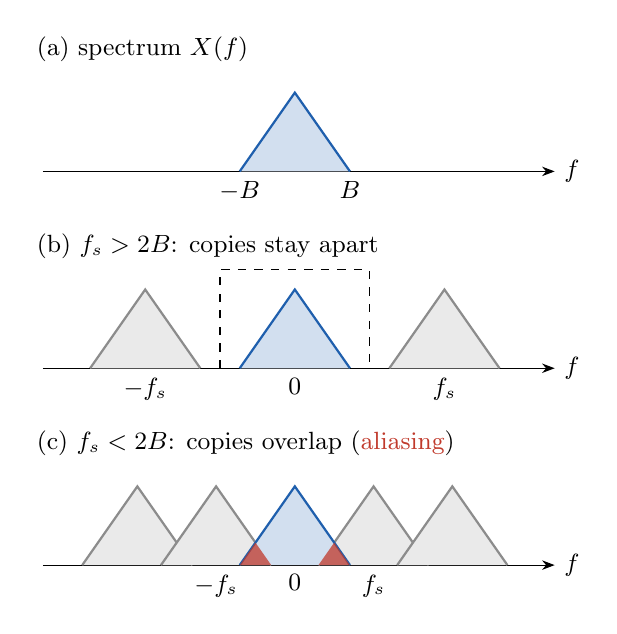
\begin{tikzpicture}[font=\small, >={Stealth[length=1.6mm]}]
  \node[anchor=west] at (-3.4,1.55) {(a) spectrum $X(f)$};
  \draw[->] (-3.2,0) -- (3.3,0) node[right] {$f$};
  \filldraw[sig, fill=sig!20, thick] (-0.7,0) -- (0,1) -- (0.7,0);
  \node[below] at (-0.7,0) {$-B$};
  \node[below] at (0.7,0) {$B$};
  \begin{scope}[yshift=-2.5cm]
    \node[anchor=west] at (-3.4,1.55) {(b) $f_s>2B$: copies stay apart};
    \draw[->] (-3.2,0) -- (3.3,0) node[right] {$f$};
    \foreach \k in {-1,1}
      \filldraw[soft, fill=soft!18, thick] ({1.9*\k-0.7},0) -- ({1.9*\k},1) -- ({1.9*\k+0.7},0);
    \filldraw[sig, fill=sig!20, thick] (-0.7,0) -- (0,1) -- (0.7,0);
    \draw[black, dashed] (-0.95,0) -- (-0.95,1.25) -- (0.95,1.25) -- (0.95,0);
    \node[below] at (-1.9,0) {$-f_s$};
    \node[below] at (0,0) {$0$};
    \node[below] at (1.9,0) {$f_s$};
  \end{scope}
  \begin{scope}[yshift=-5.0cm]
    \node[anchor=west] at (-3.4,1.55) {(c) $f_s<2B$: copies overlap (\textcolor{hot}{aliasing})};
    \draw[->] (-3.2,0) -- (3.3,0) node[right] {$f$};
    \foreach \k in {-2,-1,1,2}
      \filldraw[soft, fill=soft!18, thick] ({1.0*\k-0.7},0) -- ({1.0*\k},1) -- ({1.0*\k+0.7},0);
    \filldraw[sig, fill=sig!20, thick] (-0.7,0) -- (0,1) -- (0.7,0);
    \fill[hot, opacity=0.75] (0.3,0) -- (0.5,0.2857) -- (0.7,0) -- cycle;
    \fill[hot, opacity=0.75] (-0.3,0) -- (-0.5,0.2857) -- (-0.7,0) -- cycle;
    \node[below] at (0,0) {$0$};
    \node[below] at (1,0) {$f_s$};
    \node[below] at (-1,0) {$-f_s$};
  \end{scope}
\end{tikzpicture}
\caption{采样后的频谱。副本中心在 $kf_s$，宽 $2B$。(b) 中的虚线框是截止在 $f_s/2$ 的理想低通，用它取出中间那一份就恢复了原信号；(c) 中红色是重叠部分，即混叠。}\label{fig:spec}
\end{figure}

\subsection{采样定理}
\begin{theorem}[奈奎斯特--香农采样定理~\cite{nyquist1928,shannon1949}]
若 $X(f)=0$ 对所有 $|f|\ge B$ 成立（信号是\emph{带限}的），且 $f_s>2B$，则采样值 $\{x(nT)\}$ 唯一确定 $x(t)$，并且
\[
x(t)=\sum_n x[n]\,\sinc\Big(\frac{t-nT}{T}\Big).
\]
\end{theorem}
\begin{proof}
副本中心在 $kf_s$，各占 $(kf_s-B,\,kf_s+B)$。相邻两份不重叠当且仅当 $f_s-B\ge B$；取 $f_s>2B$ 时中间那份与其他副本之间有空隙。用理想低通 $H(f)=T\cdot\mathbf 1[|f|<f_s/2]$ 乘 $X_s(f)$，正好留下 $X(f)$。回到时域，$H$ 的逆变换是 $h(t)=T\cdot f_s\sinc(f_st)=\sinc(t/T)$，而频域相乘是时域卷积：
$x(t)=(x_s*h)(t)=\sum_n x(nT)\,h(t-nT)$，即上式。
\end{proof}

几点要讲清楚的：
\begin{itemize}
  \item \textbf{两个名字。}奈奎斯特\emph{率}（Nyquist rate）是 $2B$，是对采样率的要求；奈奎斯特\emph{频率}（Nyquist frequency）是 $f_s/2$，是给定采样率能表示的最高频率。
  \item \textbf{为什么严格大于。}$\sin(2\pi Bt)$ 以 $f_s=2B$ 采样，采样点 $t=n/(2B)$ 处 $\sin(\pi n)=0$，采到的全是零。频谱在 $\pm B$ 处恰好有能量时，等号不够。
  \item \textbf{插值公式的直觉。}第 $n$ 个 sinc 在自己的采样点等于 1、在其他采样点等于 0，所以和一定穿过每个采样点；两个采样点之间的值由所有 sinc 共同决定（图~\ref{fig:sinc}）。在所有穿过这些点的曲线里，它是唯一一条带宽不超过 $f_s/2$ 的。
  \item \textbf{历史。}惠特克（1915）给出插值公式；奈奎斯特（1928）在电报问题里发现带宽 $B$ 的信道每秒最多传 $2B$ 个独立脉冲~\cite{nyquist1928}；科捷利尼科夫（1933）独立证明了定理；香农（1949）给出今天通用的表述并放进信息论~\cite{shannon1949}。所以也叫 WKS 定理。
\end{itemize}

\begin{figure}[htbp]
\centering
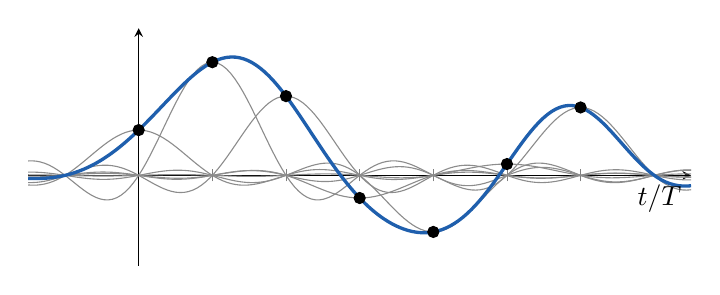
\begin{tikzpicture}[declare function={s(\t)=sin(180*\t)/(pi*\t);}]
  \begin{axis}[width=10cm, height=4.6cm, axis lines=middle, xmin=-1.5, xmax=7.5, ymin=-0.8, ymax=1.3,
      xtick={0,...,6}, xticklabels={}, ytick=\empty, xlabel={$t/T$},
      every axis x label/.style={at={(current axis.right of origin)}, anchor=north east},
      domain=-1.5:7.5, samples=158, no markers]
    \addplot[soft] {0.4*s(x)};
    \addplot[soft] {1.0*s(x-1)};
    \addplot[soft] {0.7*s(x-2)};
    \addplot[soft] {-0.2*s(x-3)};
    \addplot[soft] {-0.5*s(x-4)};
    \addplot[soft] {0.1*s(x-5)};
    \addplot[soft] {0.6*s(x-6)};
    \addplot[sig, very thick] {0.4*s(x)+1.0*s(x-1)+0.7*s(x-2)-0.2*s(x-3)-0.5*s(x-4)+0.1*s(x-5)+0.6*s(x-6)};
    \addplot[black, only marks, mark=*, mark size=2pt]
      coordinates {(0,0.4) (1,1.0) (2,0.7) (3,-0.2) (4,-0.5) (5,0.1) (6,0.6)};
  \end{axis}
\end{tikzpicture}
\caption{sinc 插值。灰线是每个采样值乘一个 sinc，蓝线是它们的和，穿过每个黑点。}\label{fig:sinc}
\end{figure}

\subsection{混叠}
若 $f_s<2B$，副本重叠，原频谱被污染，这就是\textbf{混叠}（aliasing）。最干净的例子：
\[
\cos\big(2\pi f_0\,nT\big)=\cos\big(2\pi f_0\,nT-2\pi n\big)=\cos\big(2\pi(f_0-f_s)\,nT\big).
\]
所以采样后 $f_0$ 与 $f_0-kf_s$ 无法区分，看到的频率是把 $f_0$“折回”$[-f_s/2,f_s/2]$ 后的值。$f_0=0.9f_s$ 折回后是 $-0.1f_s$：看起来是一个 $0.1f_s$ 的慢波，负号表示“方向反了”。
\begin{itemize}
  \item 电影每秒 24 帧，车轮每帧几乎转过一根辐条时，看起来就会慢慢倒转。
  \item 条纹衬衫的空间频率超过相机像素的奈奎斯特极限，折回成低频的波纹，就是摩尔纹。
  \item 斜线边缘的“锯齿”（jaggies）也是混叠。
\end{itemize}
\textbf{最重要的一点：混叠无法撤销。}采样值本身已经一模一样，任何只看采样值的算法都分不出来。唯一的办法是在采样\emph{之前}把 $f_s/2$ 以上的成分去掉。

\subsection{实际系统：滤波、采样、插值}\label{sec:recon}
\begin{itemize}
  \item \textbf{采样前：抗混叠滤波。}真实滤波器从“通过”到“截止”需要一段过渡带，所以采样率要留余量。人耳约到 20\,kHz，CD 用 44.1\,kHz 采样，奈奎斯特频率 22.05\,kHz，中间约 2\,kHz 留给过渡带。相机里的“光学低通滤镜”（OLPF）和像素本身的面积积分起同样的作用。
  \item \textbf{重建：近似的 sinc。}理想 sinc 无限长、要用到“未来”的采样、截止太陡会振铃，所以实际用短核近似。每一种插值方法都等价于一个低通滤波器（表~\ref{tab:kernels}）。
\end{itemize}

\begin{table}[htbp]
\centering
\caption{插值核的频率响应（频率以采样率为单位，$f_s=1$）。}\label{tab:kernels}
\begin{tabular}{lccc}
\toprule
核 & 频率响应 & 在 $f_s/2$ 处 & 在 $1.5f_s$ 处 \\
\midrule
理想（sinc） & 矩形 & 1 & 0 \\
最近邻（方框） & $|\sinc(f)|$ & 0.64 & 0.21 \\
线性（三角） & $\sinc^2(f)$ & 0.41 & 0.05 \\
\bottomrule
\end{tabular}
\end{table}

在 $f_s/2$ 以内就开始衰减 $\Rightarrow$ 画面变模糊；在 $f_s/2$ 以外不为零 $\Rightarrow$ 副本漏进来，表现为块状和锯齿。三次插值、Lanczos（加窗的 sinc）更接近理想，但截止越陡越容易振铃。这是一个三方权衡：模糊、漏频、振铃。

\subsection{离散时间的视角：下采样与上采样}
压缩里的采样操作大多发生在已经数字化的信号上，用离散频率更方便。对序列 $x[n]$，频率单位是“每个样本几个周期”，记作 $\nu$。因为 $n$ 是整数，$\cos(2\pi(\nu+1)n)=\cos(2\pi\nu n)$，所以只有 $\nu\in[-\tfrac12,\tfrac12]$ 可区分，最快的变化是逐点一正一负，$\nu=\tfrac12$。\textbf{这就是离散世界里的奈奎斯特极限。}

\begin{itemize}
  \item \textbf{$M$ 倍下采样}（每 $M$ 个取一个，$y[n]=x[Mn]$）在频域里是
  \[
  Y(e^{j\omega})=\frac1M\sum_{k=0}^{M-1}X\big(e^{j(\omega-2\pi k)/M}\big):
  \]
  频谱被拉宽 $M$ 倍，同时叠上 $M-1$ 个平移的副本。只有当 $x$ 的频谱在 $|\nu|<\frac1{2M}$ 以内时才不混叠，所以 2 倍下采样前要先把 $\tfrac14$ 周期/样本以上的成分滤掉。
  \item \textbf{$L$ 倍上采样}的第一步是插零（$y[Ln]=x[n]$，其余为 0），频域里 $Y(e^{j\omega})=X(e^{jL\omega})$：频谱被压缩 $L$ 倍，并出现 $L-1$ 个“镜像”（images）。第二步的插值滤波器负责去掉镜像。最近邻、双线性就是方框、三角核，所以去不干净。
\end{itemize}

\subsection{二维采样与图像}
像素网格是在水平、竖直两个方向上的采样。像素间距为 1 时，频率用 $(u,v)$ cycles/pixel 表示，能表示的范围是\textbf{奈奎斯特正方形} $|u|,|v|<\tfrac12$，采样后频谱在平面上按整数格点复制。缩小一半后极限变成 $\tfrac14$，所以\textbf{缩小图像之前必须先模糊}。

Burt 和 Adelson（1983）的\textbf{图像金字塔}~\cite{burt1983}：高斯金字塔就是反复“模糊 + 2 倍下采样”；拉普拉斯金字塔存每一层与“下一层上采样回来”的差，差值大多接近零，好压缩。论文题目就叫 \emph{The Laplacian Pyramid as a Compact Image Code}，它是采样和压缩最早的交汇之一。

工程提示：很多缩放函数默认不做抗混叠。PyTorch 的 \texttt{F.interpolate} 对双线性、双三次提供 \texttt{antialias} 参数；OpenCV 缩小时用 \texttt{INTER\_AREA} 会先做区域平均。

%======================================================================
\section{背景三：熵与无损编码}\label{sec:entropy}

\subsection{熵}
一个信源每次输出符号 $i$ 的概率是 $p_i$。出现概率为 $p$ 的事件带来的“意外程度”是 $-\log_2 p$ 比特：必然事件不带来信息，罕见事件带来很多。它的平均值就是熵~\cite{shannon1948}：
\begin{definition}[熵]
$H=-\sum_i p_i\log_2 p_i$（比特/符号）。
\end{definition}
\begin{example}
公平硬币 $H=1$；90\% 是正面的硬币 $H=-0.9\log_20.9-0.1\log_20.1\approx0.47$，这样的数据平均每个符号不到半个比特就能存下。$K$ 个等概率符号 $H=\log_2K$，这是熵的最大值。
\end{example}
越“可预测”，熵越低，越好压。压缩里的预测、变换、上下文模型，归根结底都是在降低“剩下要编码的东西”的熵。

\subsection{前缀码与信源编码定理}
给每个符号分配一个 0/1 码字。如果没有任何码字是另一个码字的前缀，解码时就不需要分隔符，叫\textbf{前缀码}。码长 $\ell_i$ 能构成前缀码的充要条件是 Kraft 不等式 $\sum_i 2^{-\ell_i}\le1$：把码字想成二叉树上的叶子，长度为 $\ell$ 的叶子占掉树的 $2^{-\ell}$。
\begin{theorem}[信源编码定理]
任何前缀码的平均码长 $L=\sum_ip_i\ell_i\ge H$；并且存在前缀码使 $L<H+1$。对 $n$ 个符号一起编码，每符号的平均码长可以任意接近 $H$。
\end{theorem}
取 $\ell_i=\lceil-\log_2p_i\rceil$ 就满足 Kraft 不等式，并给出 $L<H+1$。所以\textbf{熵是无损压缩的极限}，而且是可以逼近的。

\subsection{Huffman 编码}
Huffman（1952）~\cite{huffman1952}给出了逐符号编码时的最优前缀码：反复把概率最小的两个符号合并成一个节点，直到只剩一个根。
\begin{example}
四个符号概率 $0.5,0.25,0.125,0.125$。先合并两个 $0.125$ 得 $0.25$，再与 $0.25$ 合并得 $0.5$，最后与 $0.5$ 合并。码字 $0,10,110,111$，平均码长 $0.5\cdot1+0.25\cdot2+0.125\cdot3\cdot2=1.75$，恰好等于熵。概率都是 2 的负整数次幂时 Huffman 达到熵；否则每个符号最多多出不到 1 比特。
\end{example}
Huffman 的弱点：每个符号至少 1 比特。对概率 0.99 的符号（比如 JPEG 里大量的零），理想码长只有 0.015 比特。JPEG 的办法是把“一串零”合成一个符号（游程编码，第~\ref{sec:jpeg}~节）。

\subsection{算术编码与上下文模型}
算术编码把整条消息映射成 $[0,1)$ 中的一个区间：每读一个符号，就按它的概率把当前区间切一刀、留下对应的那一段。最后的区间长度等于整条消息的概率 $P$，写下这个区间里的一个数大约需要 $-\log_2P+2$ 比特。于是\textbf{码长几乎正好是负对数概率}，没有“每符号至少 1 比特”的限制。

算术编码把“建模”和“编码”分开了：只要你能给出每个符号的概率，编码器就能以接近 $-\log_2 p$ 的代价写下它。\textbf{概率估得越准，比特越少。}后来的编码器都用上下文自适应的算术编码（H.264/HEVC 的 CABAC，JPEG 2000 的 MQ 编码器），学习型编码器（第~\ref{sec:learned}~节）则用神经网络来给出这个概率。

%======================================================================
\section{背景四：率失真理论}\label{sec:rd}

\subsection{有损压缩的极限}
无损压缩的极限是熵。有损压缩允许重建 $\hat X$ 与 $X$ 有差别，用一个失真度量（通常是均方误差 $d=(X-\hat X)^2$）衡量。香农 1959 年~\cite{shannon1959}定义了：
\begin{definition}[率失真函数]
\[
R(D)=\min_{p(\hat x|x):\ \mathbb E[d(X,\hat X)]\le D} I(X;\hat X),
\]
即平均失真不超过 $D$ 时，每个样本最少需要的比特数。
\end{definition}
这里的互信息 $I(X;\hat X)$ 是“重建里包含了多少关于原信号的信息”。定理说：比特率高于 $R(D)$ 就存在编码器达到失真 $D$（对很长的样本块一起编码），低于 $R(D)$ 则不可能。和熵一样，它是一个\emph{极限}，不告诉你具体怎么造编码器（香农的证明用的是随机码本）。

\subsection{高斯信源与“每比特 6 分贝”}
\begin{theorem}
方差为 $\sigma^2$ 的高斯信源，均方误差失真下
\[
R(D)=\tfrac12\log_2\frac{\sigma^2}{D}\quad(0<D\le\sigma^2),\qquad\text{即}\quad D(R)=\sigma^2\,2^{-2R}.
\]
\end{theorem}
\textbf{直觉。}每多 1 比特，就能把每个取值区间再切成两半，误差的标准差减半，方差变成 $1/4$，信噪比提高 $10\log_{10}4\approx6.02$\,dB。\textbf{“每比特 6 分贝”}是信号处理里最常用的经验法则之一。
\textbf{另一个事实：}同方差的信源里，高斯在均方误差下最难压（它的熵最大）。所以高斯的 $R(D)$ 对任何同方差信源都是一个上界式的参考。

\subsection{标量量化离极限有多远}
最简单的有损编码是均匀量化：步长 $\Delta$，把每个值四舍五入到最近的格点。步长较小时，误差近似在 $[-\Delta/2,\Delta/2]$ 上均匀分布，方差 $\Delta^2/12$。再用熵编码写下量化后的整数，高码率时可以证明，它与率失真极限只差一个常数：
\[
\frac{D_{\text{均匀量化+熵编码}}}{D_{\text{极限}}}\to\frac{\pi e}{6}\approx1.42,\quad\text{即约 }1.53\text{\,dB，或每样本 }0.254\text{ 比特}.
\]
这说明：\textbf{在高码率下，“好的变换 + 均匀量化 + 好的熵编码”几乎就是最优的}，剩下的差距来自“逐样本量化”而不是“整块一起量化”。这是变换编码能统治几十年的理论原因。

\subsection{多个分量怎么分比特：反向注水}\label{sec:rwf}
设有 $n$ 个独立的高斯分量，方差 $\sigma_1^2,\dots,\sigma_n^2$，总失真预算 $\sum D_i=D$。要最小化总比特数 $\sum_i\tfrac12\log_2^{+}(\sigma_i^2/D_i)$。
\begin{theorem}[反向注水]
存在一个“水位”$\theta$，使最优分配为
\[
D_i=\min(\theta,\sigma_i^2),\qquad R_i=\max\Big(0,\ \tfrac12\log_2\frac{\sigma_i^2}{\theta}\Big),
\]
$\theta$ 由 $\sum_iD_i=D$ 决定~\cite{cover2006}。
\end{theorem}
\begin{proof}[（直觉）]
对 $D_i$ 求导：$\partial R_i/\partial D_i=-1/(2\ln2\,D_i)$。拉格朗日条件要求所有“还在花比特”的分量边际收益相同，于是它们的 $D_i$ 相等，记作 $\theta$。但 $D_i$ 不能超过 $\sigma_i^2$（什么都不传，误差就是方差本身）：方差小于 $\theta$ 的分量被截在 $D_i=\sigma_i^2$，即一个比特都不给。
\end{proof}
画成图就是：把各分量的方差画成高低不同的柱子，倒入“水”到高度 $\theta$。水面以下的部分是误差，高出水面的部分才花比特。\textbf{比特越少，水位越高，被整个丢掉的分量越多。}

\subsection{平稳过程：在频谱上注水}\label{sec:waterfill}
平稳高斯过程的不同频率分量（在长时长下）近似不相关、因而近似独立，于是功率谱 $S(f)$ 扮演 $\sigma_i^2$ 的角色（Kolmogorov 1956~\cite{kolmogorov1956}，Berger 1971~\cite{berger1971}）：
\[
D_\theta=\int\min\{\theta,S(f)\}\,\mathrm df,\qquad R_\theta=\int\tfrac12\log_2^{+}\frac{S(f)}{\theta}\,\mathrm df.
\]
对功率谱从低频往高频单调下降的信号（比如图像），$S(f)>\theta$ 的集合就是一个低频带 $|f|<f_\theta$。于是：

\begin{alertblock}{关键结论}
在率失真意义下，最优的有损编码只对 $|f|<f_\theta$ 的频率花比特，其余直接置零。\textbf{它本身就是一个截止在 $f_\theta$ 的低通滤波器}；比特越少，$f_\theta$ 越小。这是第 23 页的内容，也是整场“联系”部分的支点。
\end{alertblock}

\begin{figure}[htbp]
\centering
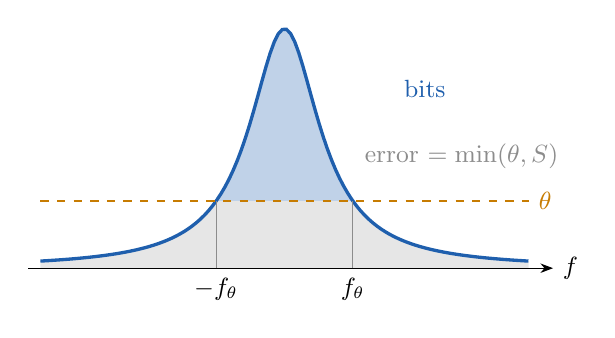
\begin{tikzpicture}[x=1.55cm, y=1.9cm, font=\small, >={Stealth[length=1.6mm]},
    declare function={S(\t)=1.6/(1+(\t/0.35)^2);}]
  \fill[soft!22] (-2,0) -- plot[domain=-2:-0.56, samples=50] (\x,{S(\x)}) -- (0.56,0.45)
    -- plot[domain=0.56:2, samples=50] (\x,{S(\x)}) -- (2,0) -- cycle;
  \fill[sig!28] (-0.56,0.45) -- plot[domain=-0.56:0.56, samples=60] (\x,{S(\x)}) -- cycle;
  \draw[sig, very thick] plot[domain=-2:2, samples=120] (\x,{S(\x)});
  \draw[accent, thick, dashed] (-2,0.45) -- (2,0.45) node[right] {$\theta$};
  \draw[->] (-2.1,0) -- (2.2,0) node[right] {$f$};
  \draw[soft] (-0.56,0) -- (-0.56,0.45);
  \draw[soft] (0.56,0) -- (0.56,0.45);
  \node[below] at (-0.56,0) {$-f_\theta$};
  \node[below] at (0.56,0) {$f_\theta$};
  \node[sig] at (1.15,1.2) {bits};
  \node[soft] at (1.45,0.75) {error $=\min(\theta,S)$};
\end{tikzpicture}
\caption{在频谱上反向注水。蓝色阴影是花比特的部分，灰色是误差。只有 $|f|<f_\theta$ 被编码。}\label{fig:rwf}
\end{figure}

\subsection{一个干净的计算：$1/f^2$ 谱}\label{sec:onef}
取一维、理想的 $S(f)=1/f^2$。水位 $\theta=1/f_\theta^2$，被编码的频带是 $|f|<f_\theta$，
\[
R=\int_{-f_\theta}^{f_\theta}\tfrac12\log_2\frac{f_\theta^2}{f^2}\,\mathrm df=2\int_0^{f_\theta}\log_2\frac{f_\theta}{f}\,\mathrm df=\frac{2f_\theta}{\ln2}
\]
（用到 $\int_0^a\ln(a/f)\,\mathrm df=a$）。这个频带需要的采样率是 $2f_\theta$，所以
\[
\frac{R}{2f_\theta}=\frac1{\ln2}\approx1.44\ \text{比特/样本，与码率无关.}
\]
二维时 $S\propto1/\rho^2$（$\rho$ 是径向频率），被编码的是半径 $\rho_\theta$ 的圆盘，$R=\pi\rho_\theta^2/(2\ln2)$，需要的样本密度等于圆盘面积 $\pi\rho_\theta^2$，每个保留样本约 $1/(2\ln2)\approx0.72$ 比特。

\textbf{怎么理解：}对这种理想信源，码率翻倍时，最优编码不是让每个样本更精确，而是\emph{保留更多的样本}（更宽的频带、更高的分辨率），每个样本分到的比特数不变。这是“比特少就少采样”最直观的数学版本。注意它是高斯、精确 $1/f^2$ 的理想化结果，0.72 不是真实图像的数字，不要当实测数据引用。

%======================================================================
\section{背景五：变换编码}\label{sec:transform}

\subsection{为什么要变换}
相邻像素高度相关（自然图像相邻像素的相关系数约 0.95）。直接逐像素量化，每个像素都要花差不多的比特，浪费在“可以从邻居猜出来”的部分上。变换编码的思路：先用一个\textbf{正交变换}把相关的像素变成不相关的系数，让能量集中到少数几个系数上，再按反向注水的精神分配比特。
\begin{definition}[变换编码增益]
$N$ 个系数方差为 $\sigma_k^2$ 时，高码率下最优比特分配比直接量化省下的倍数是
\[
G=\frac{\frac1N\sum_k\sigma_k^2}{\big(\prod_k\sigma_k^2\big)^{1/N}}\quad(\text{算术平均}/\text{几何平均}).
\]
\end{definition}
正交变换保持总能量（分子不变），能量越集中，几何平均越小，增益越大。最优比特分配（Huang \& Schultheiss 1963~\cite{huang1963}）是
$R_k=\bar R+\tfrac12\log_2\big(\sigma_k^2/(\prod_j\sigma_j^2)^{1/N}\big)$：方差大一倍，多给半个比特。这正是高码率下的反向注水；低码率时 $R_k$ 算出来为负的分量，就直接置零。

\subsection{KLT 与 DCT}
使系数完全不相关、并且增益最大的正交变换是 \textbf{KLT}：协方差矩阵的特征向量。它依赖数据，每类图像都要算，还要把变换本身传给解码器。

对一阶马尔可夫信号（相邻相关系数 $\rho$，相距 $k$ 的相关系数 $\rho^{|k|}$），当 $\rho\to1$ 时 KLT 趋近\textbf{离散余弦变换}（DCT，Ahmed、Natarajan、Rao 1974~\cite{ahmed1974}）。自然图像的 $\rho\approx0.95$，所以固定的 DCT 几乎和 KLT 一样好，而且有快速算法。正交归一的一维 DCT（$N=8$）：
\[
c_k=\alpha_k\sum_{n=0}^{N-1}x_n\cos\Big[\frac{\pi}{N}\Big(n+\frac12\Big)k\Big],\qquad\alpha_0=\sqrt{1/N},\ \alpha_k=\sqrt{2/N}.
\]
二维 DCT 可分离：先对每行做，再对每列做，得到 64 个“基图像”的系数。左上角的 $c_{00}$ 叫 DC（块的平均亮度），其余叫 AC。

\textbf{为什么不用 DFT？}DFT 隐含把块周期延拓，块左右边缘的值不同就产生跳变，能量泄漏到高频。DCT 对应偶对称延拓，边界连续，系数衰减更快；而且是实数运算。

\subsection{量化}
均匀量化：$\hat c=\Delta\cdot\mathrm{round}(c/\Delta)$。$|c|<\Delta/2$ 的系数变成 0。很多编码器用“死区”量化器，把零附近的区间放宽，让更多小系数变成零，因为零在熵编码里几乎不花比特。\textbf{量化是整个流水线里唯一丢信息的一步}：变换可逆，熵编码可逆。

%======================================================================
\section{背景六：JPEG}\label{sec:jpeg}

JPEG（1992）~\cite{wallace1992}至今仍是最常用的图像格式。把它的每一步和前面的理论对上，是讲好第二部分的关键。

\subsection{颜色：YCbCr 与 4:2:0}
先把 RGB 转成亮度与色度：$Y=0.299R+0.587G+0.114B$，$C_b$、$C_r$ 分别是蓝、红与亮度的差（加偏移）。好处有二：三个通道去相关；把人眼最敏感的亮度单独分出来。

\textbf{色度 4:2:0}：$C_b$、$C_r$ 先低通，再横竖各 2 倍下采样，各剩 $1/4$ 的样本。每像素的样本数从 3 变成 $1+\tfrac14+\tfrac14=1.5$，一步减半。依据是人眼的\textbf{对比敏感度函数}（CSF）：对颜色细节的截止频率远低于亮度。对人眼而言，色度本来就是“带限”的，按更低的采样率采样不损失可见信息。\emph{这是 JPEG 里唯一真正降低采样率的一步。}

\subsection{分块 DCT 与量化表}
把每个通道切成 $8\times8$ 的块，每块做二维 DCT，得到 64 个系数。然后每个系数除以量化表里对应的步长再取整：
\[
\hat c_{uv}=Q_{uv}\cdot\mathrm{round}(c_{uv}/Q_{uv}).
\]
标准附录给出的亮度表示例（幻灯片第 14 页）左上角步长 10--16，右下角高频到 100 以上，是按人眼对不同空间频率的可见度调出来的。高频步长大，大多数高频系数被量化成零。\textbf{这就是手工做的反向注水：小于半个步长的系数一个比特都不花。}

“质量因子”$q$ 是整体缩放这张表。常见实现（libjpeg）的做法：$q<50$ 时乘 $50/q$，$q\ge50$ 时乘 $(200-2q)/100$。$q=50$ 用原表，$q=100$ 步长都变成 1。

为什么是 $8\times8$：块太小，能量集中得不够；块太大，块内内容不再“平稳”，计算量也大（1990 年代的硬件）。HEVC、AV1 都改成了可变块大小。

\subsection{熵编码}
\begin{enumerate}
  \item \textbf{DC 系数}：相邻块的平均亮度很接近，所以存与前一块 DC 的差（DPCM）。
  \item \textbf{Z 字形扫描}：按从低频到高频的顺序把 63 个 AC 系数排成一行，零大多聚在末尾。
  \item \textbf{游程编码}：每个非零系数记成（前面有几个零，这个值的位数）加上值本身的二进制位；一串零连到块尾时用一个“块结束”（EOB）符号。这样就把 Huffman“每符号至少 1 比特”的问题绕开了：一长串零只花几个比特。
  \item \textbf{Huffman 编码}这些符号。
\end{enumerate}

\subsection{失真：块效应与振铃}\label{sec:artifacts}
\begin{itemize}
  \item \textbf{块效应}：每个块独立量化，低码率时相邻块的 DC 和低频系数对不上，出现方格。
  \item \textbf{振铃}：截掉一个块的高频系数，等于在频域乘一个（近似的）矩形窗，即在空间域与一个 sinc 型函数卷积，sinc 的旁瓣就成了边缘两侧的波纹，叫“蚊式噪声”。
\end{itemize}
振铃背后是\textbf{吉布斯现象}：对一个跳变做傅里叶部分和，跳变两侧的过冲约为跳变高度的 9\%（精确值约 8.95\%），并且保留的频率再多，过冲也不变小，只是波纹区域变窄（图~\ref{fig:gibbs}）。

\begin{figure}[htbp]
\centering
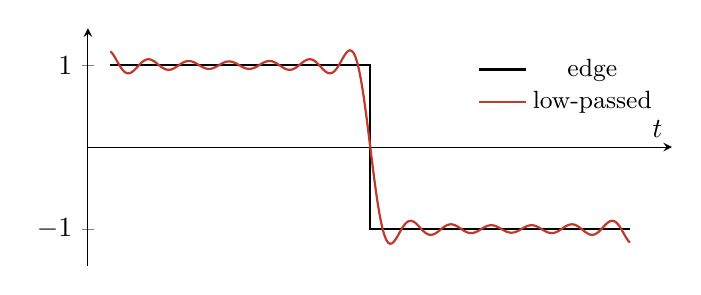
\begin{tikzpicture}
  \begin{axis}[width=9cm, height=4.6cm, axis lines=middle, xmin=0, xmax=6.5, ymin=-1.45, ymax=1.45,
      xtick=\empty, ytick={-1,1}, xlabel={$t$}, no markers,
      legend style={draw=none, fill=none, font=\small, at={(0.99,0.92)}, anchor=north east}]
    \addplot[black, thick, const plot] coordinates {(0.25,1) (3.1416,-1) (6.03,-1)};
    \addlegendentry{edge}
    \addplot[hot, thick, domain=0.25:6.03, samples=300]
      {4/pi*(sin(deg(x)) + sin(deg(3*x))/3 + sin(deg(5*x))/5 + sin(deg(7*x))/7 + sin(deg(9*x))/9 + sin(deg(11*x))/11 + sin(deg(13*x))/13)};
    \addlegendentry{low-passed}
  \end{axis}
\end{tikzpicture}
\caption{吉布斯现象：方波只保留 7 个奇次谐波的部分和，边缘两侧出现约 9\% 的过冲和波纹。}\label{fig:gibbs}
\end{figure}

\begin{alertblock}{别讲错}
JPEG 丢掉高频系数是块内的\emph{带限}（低通），\textbf{不是}降低采样率：图像的像素数没有变。真正降低采样率的是色度 4:2:0、先缩小再编码、AV1 的超分辨率编码。不要说“JPEG 丢高频就是遵循奈奎斯特”。
\end{alertblock}

%======================================================================
\section{背景七：小波与 JPEG 2000}\label{sec:wavelet}

\subsection{多分辨率的想法}
DCT 的问题是固定块：块太大，边缘附近的高频会“漫”到整个块；块太小，平坦区域的能量集中不够。小波（Mallat 1989~\cite{mallat1989}）换个思路：对整幅图做多分辨率分解，低频用大尺度、高频用小尺度，没有块。

\subsection{最简单的例子：Haar}
每两个相邻样本 $(x_{2n},x_{2n+1})$ 变成
\[
a_n=\frac{x_{2n}+x_{2n+1}}{\sqrt2}\ (\text{平均，低频}),\qquad d_n=\frac{x_{2n}-x_{2n+1}}{\sqrt2}\ (\text{差，高频}).
\]
两个数进、两个数出，可逆：$x_{2n}=(a_n+d_n)/\sqrt2$，$x_{2n+1}=(a_n-d_n)/\sqrt2$。这叫\textbf{临界采样}（总样本数不变）加\textbf{完美重建}。对平坦区域，$d_n\approx0$，几乎不花比特；只有边缘处 $d_n$ 大。再对 $a_n$ 重复，就得到多级分解。

\subsection{两通道滤波器组与混叠抵消}
一般地，用低通 $H_0$、高通 $H_1$ 把信号分成两半频带，各自 2 倍下采样；重建时各自插零上采样，再用 $G_0$、$G_1$ 滤波后相加（图~\ref{fig:fb}）。

\begin{figure}[htbp]
\centering
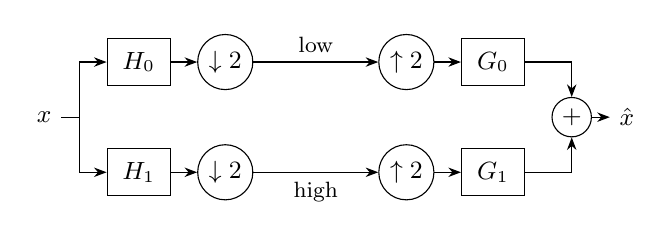
\begin{tikzpicture}[font=\small, >={Stealth[length=1.6mm]},
    f/.style={draw, minimum width=8mm, minimum height=6mm, inner sep=1pt},
    r/.style={draw, circle, inner sep=0pt, minimum size=7mm}]
  \node (x) at (0,0) {$x$};
  \node[f] (h0) at (1.2,0.7) {$H_0$};
  \node[f] (h1) at (1.2,-0.7) {$H_1$};
  \node[r] (d0) at (2.3,0.7) {$\downarrow 2$};
  \node[r] (d1) at (2.3,-0.7) {$\downarrow 2$};
  \node[r] (u0) at (4.6,0.7) {$\uparrow 2$};
  \node[r] (u1) at (4.6,-0.7) {$\uparrow 2$};
  \node[f] (g0) at (5.7,0.7) {$G_0$};
  \node[f] (g1) at (5.7,-0.7) {$G_1$};
  \node[draw, circle, inner sep=0pt, minimum size=5mm] (s) at (6.7,0) {$+$};
  \node (y) at (7.4,0) {$\hat x$};
  \draw[->] (x) -- (0.45,0) |- (h0);
  \draw[->] (0.45,0) |- (h1);
  \draw[->] (h0) -- (d0);
  \draw[->] (h1) -- (d1);
  \draw[->] (d0) -- node[above, font=\footnotesize] {low} (u0);
  \draw[->] (d1) -- node[below, font=\footnotesize] {high} (u1);
  \draw[->] (u0) -- (g0);
  \draw[->] (u1) -- (g1);
  \draw[->] (g0) -| (s);
  \draw[->] (g1) -| (s);
  \draw[->] (s) -- (y);
\end{tikzpicture}
\caption{两通道滤波器组：分析端 $H_0,H_1$ 加 $\downarrow2$，综合端 $\uparrow2$ 加 $G_0,G_1$。编码器在中间对两路量化、编码。}\label{fig:fb}
\end{figure}

用 $z$ 变换分析。先 $\downarrow2$ 再 $\uparrow2$ 的结果是 $\tfrac12[X(z)+X(-z)]$，其中 $X(-z)$ 是频谱平移了半个采样率，也就是\textbf{混叠项}。整个系统的输出是
\[
\hat X(z)=\tfrac12\big[H_0(z)G_0(z)+H_1(z)G_1(z)\big]X(z)+\tfrac12\big[H_0(-z)G_0(z)+H_1(-z)G_1(z)\big]X(-z).
\]
取 $G_0(z)=H_1(-z)$、$G_1(z)=-H_0(-z)$，第二个方括号恒为零：\textbf{两路的混叠大小相等、符号相反，正好抵消}。再让第一个方括号等于 $2z^{-\ell}$，就是完美重建（只延迟 $\ell$ 个样本）。Haar 验算：$H_0=(1+z^{-1})/\sqrt2$，$H_1=(1-z^{-1})/\sqrt2$，第一个方括号 $=\tfrac12[(1+z^{-1})^2-(1-z^{-1})^2]=2z^{-1}$。

这是采样理论在压缩里最漂亮的一次应用：每一路单独看都违反了采样定理（滤波器不是理想半带），但整体上信息一点不丢。

\subsection{JPEG 2000}
JPEG 2000（2000）~\cite{skodras2001}对行、列各做一次分解，得到 LL、HL、LH、HH 四个子带，再对 LL 重复。它用 CDF 9/7 小波（有损）和 LeGall 5/3 小波（整数运算，可无损）。量化后，EBCOT 把每个子带切成小的码块，按位平面从高到低编码，配合 MQ 算术编码器。结果是\textbf{嵌入式码流}：在任何位置截断都能解出一幅质量较低的图；只解码低频子带就得到 $1/2$、$1/4$ 分辨率的图。它没能取代 JPEG（复杂度高，JPEG 已经够用），但在数字电影和医学影像里是标准格式。

%======================================================================
\section{背景八：借用视频编码的图像格式}\label{sec:video}

2010 年以后，最好的图像格式都来自视频编码的“帧内编码”：WebP（有损部分即 VP8 帧内），HEIC（HEIF 容器里的 HEVC 帧内，苹果设备 2017 年起默认），AVIF（AV1 帧内，2019）。新工具有：
\begin{itemize}
  \item \textbf{帧内预测}：每个块先用已经解码的上方、左方像素沿某个方向外推出来，只对\emph{残差}做变换和量化。HEVC 有 35 种模式（平面、DC 和 33 个角度），VVC 有 67 种；AV1 也有几十种方向，并能由亮度预测色度（CfL）。预测把“能猜到的”去掉，残差的熵更低。
  \item \textbf{可变块大小}（从 $4\times4$ 到 $64\times64$ 甚至更大），平坦区域用大块，细节区域用小块。
  \item \textbf{多种变换}：DCT 之外还有 DST 等，按残差的统计选择。
  \item \textbf{上下文自适应算术编码}（CABAC）。
  \item \textbf{环路滤波}：去块滤波、样本自适应偏移等，专门压掉块效应和振铃。
\end{itemize}
“通常比 JPEG 小 30\%--50\%”是常见的粗略说法，具体取决于图片和质量指标。

%======================================================================
\section{背景九：学习型压缩}\label{sec:learned}

\subsection{结构}
Ballé 等（2017）~\cite{balle2017}把整个编码器换成神经网络，并端到端训练。结构与 JPEG 一一对应：
\begin{itemize}
  \item \textbf{分析变换} $g_a$（对应 DCT）：几层卷积，每层步长 2，共 4 次，得到隐变量 $y$，空间尺寸是原图的 $1/16$，通道数如 192。
  \item \textbf{量化} $\hat y=\mathrm{round}(y)$。
  \item \textbf{熵模型} $p(\hat y)$：给每个量化值一个概率，交给算术编码器，码长约 $-\log_2p(\hat y)$。
  \item \textbf{综合变换} $g_s$（对应逆 DCT）：重建 $\hat x$。
\end{itemize}
训练目标是率失真的拉格朗日形式：
\[
\mathcal L=R+\lambda D=\mathbb E\big[-\log_2p(\hat y)\big]+\lambda\,\mathbb E\|x-\hat x\|^2,
\]
$\lambda$ 控制压缩率与质量的权衡，通常每个 $\lambda$ 训练一个模型。和普通自编码器的区别：普通自编码器只压维度，不管比特；压缩要真正数比特，所以必须有量化和熵模型，并把码率写进损失。

\subsection{让它能训练、能变好的三个技术}
\begin{enumerate}
  \item \textbf{取整不可导。}训练时用 $\tilde y=y+u$，$u\sim U(-\tfrac12,\tfrac12)$ 代替 $\mathrm{round}(y)$。这与“量化误差近似均匀、独立的噪声”的模型一致，Widrow 的量化定理（第~\ref{sec:widrow}~节）给出了这个模型成立的条件。从概率的角度看，整个系统可以解释成一个变分自编码器，码率项就是 KL 散度。
  \item \textbf{超先验}（Ballé 等 2018~\cite{balle2018}）。固定的 $p(\hat y)$ 不知道图里哪里是天空、哪里是纹理。超先验再用一个小网络 $h_a$ 从 $y$ 提取边信息 $z$，量化后传过去（比特很少）；解码端 $h_s$ 从 $z$ 预测每个 $y_i$ 的尺度 $\sigma_i$，熵模型据此给出更准的概率。\emph{概率估得越准，比特越少}（第~\ref{sec:entropy}~节）。
  \item \textbf{上下文模型}（Minnen 等 2018~\cite{minnen2018}）。按顺序解码，用已经解码的邻居预测当前 $y_i$ 的分布，和帧内预测是同一个想法。代价是串行解码慢，后来有棋盘格、按通道分组等并行化方案。
\end{enumerate}
到 2020 年，这类方法在 PSNR 上与 VVC 帧内编码相当（Cheng 等~\cite{cheng2020}）。2025 年，JPEG AI（ISO/IEC 6048-1:2025）~\cite{jpegai2025}成为第一个基于学习的图像编码国际标准，目标同时服务人眼观看和机器视觉任务。没能马上取代 JPEG 的原因：解码要跑神经网络，手机上耗电耗时；熵模型在不同硬件上的浮点结果必须完全一致，否则算术解码会出错。

\subsection{失真之外：感知}
\textbf{均方误差低，不等于看起来真实。}当码率低、解码器不确定细节是什么时，均方误差最小的答案是“所有可能细节的条件平均”，平均出来就是模糊。Blau 和 Michaeli（2018）~\cite{blau2018}把“感知质量”定义为重建图像分布与真实图像分布之间的距离，证明了\textbf{感知--失真权衡}：在失真很低的区域，感知质量必然变差，反之亦然；并且要求“分布完全一样”时，均方误差最多是最小均方误差的两倍。2019 年他们把码率加进来，得到率--失真--感知三方权衡~\cite{blau2019}。

于是有了\textbf{生成式解码器}：用 GAN（HiFiC，Mentzer 等 2020~\cite{mentzer2020}）或条件扩散模型（Yang \& Mandt 2023~\cite{yang2023}）在低码率下生成逼真的纹理，PSNR 反而略低。要讲清楚的一点：\textbf{这些细节是生成的，不是传过来的}。拍照、社交媒体可以，医学、取证图像就不行。

\subsection{怎么比较编码器}
\begin{itemize}
  \item \textbf{PSNR} $=10\log_{10}(255^2/\mathrm{MSE})$：简单，但对模糊不敏感。
  \item \textbf{SSIM / MS-SSIM}~\cite{wang2003}：比较局部的亮度、对比度和结构，多尺度版本更稳。
  \item \textbf{LPIPS}~\cite{zhang2018}：比较深度网络特征之间的距离，更接近人的判断。
  \item \textbf{FID}：比较两组图像在特征空间里的分布，衡量“真实感”，用于生成式编码器。
  \item \textbf{BD-rate}（Bjøntegaard 2001~\cite{bjontegaard2001}）：对两条“码率--PSNR”曲线（码率取对数），在共同的质量区间上拟合并积分，求同等质量下码率的平均相对差，负数表示省比特。“比 X 省 30\%”的说法通常就是 BD-rate $=-30\%$。
\end{itemize}
换一个指标，编码器的排名可能就变了，生成式编码器在 PSNR 下往往吃亏。所以看任何“省了多少”的数字，先问是什么指标、什么测试集。

%======================================================================
\section{背景十：采样与压缩在哪里相遇}\label{sec:link}

这一节是第三部分（第 22--27 页）的依据。每条联系都标了证据类型：\textbf{定理}、\textbf{实验}或\textbf{工程实践}。演讲时只讲结论，但被追问时要能说出出处和条件。

\subsection{香农的 $2WT$：先数样本，再数比特（定理）}
香农 1949 年的论文 \emph{Communication in the presence of noise}~\cite{shannon1949}正是采样定理的经典出处。他证明采样定理的目的，是说明“带宽 $W$、时长 $T$ 的信号大约由 $2WT$ 个数确定”，于是一个信号就是 $2WT$ 维空间里的一个点；接着他在这个几何图像上算出了信道容量 $C=W\log_2(1+S/N)$。所以在香农自己的框架里，\textbf{采样就是“把波形变成有限维向量”的那一步，比特是在这之后才计算的}。“比特率 = 采样率 $\times$ 每样本比特数”不是比喻，而是这个框架的直接推论。

例：$4000\times3000$ 的照片有 $1.2\times10^7$ 个像素，平均每像素 1 比特就是 $1.2\times10^7$ 比特 $=1.5$\,MB。

\subsection{最优有损编码本身是一个低通（定理）}
见第~\ref{sec:waterfill}~节。要点重复一遍：在比特预算 $R$ 下，最优编码只对 $S(f)>\theta$ 的频率花比特。图像的谱从低频往高频下降，所以这就是一个低频带 $|f|<f_\theta$，比特越少，$f_\theta$ 越小。JPEG 的量化表把高频系数量化成零，是这件事的手工近似；第~\ref{sec:onef}~节的 $1/f^2$ 计算说明，对理想信源，码率增加时最优编码是“保留更多样本”，而不是“让每个样本更精确”。

\subsection{比特受限时，低于奈奎斯特采样（定理 + 实验 + 工程实践）}
\begin{itemize}
  \item \textbf{定理。}Kipnis、Goldsmith、Eldar、Weissman（2016）~\cite{kipnis2016}研究“先以采样率 $f_s$ 采样（可以低于奈奎斯特），再用每秒 $R$ 比特编码”的联合问题，给出采样率、码率、失真三者的关系。结论之一：对每个码率 $R$，存在一个\textbf{临界采样率} $f_R$，等于反向注水中 $S(f)>\theta$ 的那部分频率的总宽度（对单峰对称谱就是 $2f_\theta$）。以 $f_R$（配合合适的采样前滤波）采样，就已经能达到不采样时的最优失真 $D(R)$，再提高采样率也没有好处。谱能量越集中，$f_R$ 比奈奎斯特率低得越多。Kipnis、Eldar、Goldsmith 在 \emph{IEEE Signal Processing Magazine}（2018）~\cite{kipnis2018}上把它写成了综述，题目就叫 \emph{Analog-to-digital compression}。
  \item \textbf{实验。}Bruckstein、Elad、Kimmel（2003）~\cite{bruckstein2003}：先把图像缩小，用 JPEG 压缩小图，解码后再插值放大，\textbf{在低码率下 PSNR 比直接用 JPEG 压缩原图更高}；最优缩小倍数可以从图像的自相关估计出来。这是上面定理在图像上的实验版本。
  \item \textbf{工程实践。}AV1 的\textbf{帧超分辨率}~\cite{av1overview}：编码器可以把一帧在水平方向缩小（缩放比 8/9 到 8/16，即最多 2 倍）后编码，解码器在环路里先线性上采样，再用环路恢复滤波器补回一部分细节；只做水平方向是为了硬件便宜。VVC 的参考图像重采样允许码流中途切换分辨率。流媒体服务把每个片源按多种分辨率和码率编码，画出“质量--码率”曲线，取所有分辨率的上包络：低码率时包络上的点来自低分辨率（Netflix 2015~\cite{netflix2015}）。
\end{itemize}
\begin{alertblock}{这一页的一句话}
既然高于 $f_\theta$ 的频率反正不编码，就不必为它们采样。比特少的时候，少采样反而更好。
\end{alertblock}
它和第一部分并不矛盾：降低采样率之前仍然要先低通，否则混叠。区别只在于，比特受限时这个低通几乎“免费”，因为最优编码本来就要丢掉那些频率。

\subsection{编解码器内部的采样操作（工程实践）}
\begin{table}[htbp]
\centering
\caption{编解码器里的采样操作。}\label{tab:inside}
\begin{tabular}{lll}
\toprule
在哪里 & 采样操作 & 对应第一部分的哪个想法 \\
\midrule
JPEG、视频 & 色度 4:2:0 & 对人眼而言色度是带限的 \\
JPEG 2000 & 半带滤波 $+\downarrow2$，逐级 & 混叠恰好抵消（第~\ref{sec:wavelet}~节） \\
JPEG 2000 & 只解码低频子带 & 事后选一个更低的采样率 \\
AV1、VVC & 以较低分辨率编码 & 比特受限时低于奈奎斯特 \\
学习型编码器 & 步长 2 的卷积 $\downarrow2$、$\uparrow2$ & 学出来的金字塔 \\
JPEG & 高频系数置零 & 低通（不是降采样）$\Rightarrow$ 振铃 \\
\bottomrule
\end{tabular}
\end{table}

\subsection{以稀疏性代替带限：压缩感知与有限新息率（定理 + 应用）}
采样定理的先验是“带限”。压缩领域发现了另一种更强的先验：\textbf{稀疏}。一个长度为 $n$ 的向量，如果在某组基（DCT、小波）下只有 $k\ll n$ 个系数明显不为零，就叫 $k$-稀疏。自然图像是近似稀疏的，这正是变换编码有效的原因。

\begin{theorem}[压缩感知，非正式~\cite{candes2006,donoho2006}]
若 $x\in\mathbb R^n$ 在某组基下 $k$-稀疏，用一个 $m\times n$ 的随机测量矩阵 $\Phi$ 得到 $y=\Phi x$，只要 $m\ge Ck\log(n/k)$，就能以很高的概率通过求解
\[
\min_x\|x\|_1\quad\text{s.t.}\quad y=\Phi x
\]
精确恢复 $x$（有噪声时稳定地近似恢复）。
\end{theorem}
几点理解：
\begin{itemize}
  \item 为什么用 $\ell_1$：直接最小化非零个数（$\ell_0$）是组合爆炸问题；$\ell_1$ 是它的凸松弛，几何上“菱形的角”恰好落在稀疏向量上。
  \item 为什么要随机：随机矩阵以高概率满足“受限等距性质”（RIP），即几乎保持所有稀疏向量的长度，不同的稀疏信号不会被映射到同一个测量。
  \item Donoho 论文的出发点正是压缩：既然大部分样本采集之后马上被变换编码丢掉，为什么不一开始就只采集需要的那部分？它把\emph{压缩用的先验}搬到了\emph{采样}这一步。
\end{itemize}
\textbf{应用。}单像素相机（Duarte 等 2008~\cite{duarte2008}）用一个数字微镜阵列随机调制光线，一个探测器测很多次，就重建出一幅图；它在红外、太赫兹这类“单个探测器很贵”的波段有用。磁共振成像本来就在频域（k 空间）采样，每一条线都要时间；在 k 空间随机欠采样、再用小波稀疏性重建，可以把扫描缩短数倍（Lustig、Donoho、Pauly 2007~\cite{lustig2007}）。2017 年，Siemens 和 GE 的压缩感知 MRI 技术获得美国 FDA 许可，厂商称心脏电影成像可以从数分钟缩短到十几秒。

\textbf{有限新息率}（Vetterli、Marziliano、Blu 2002~\cite{vetterli2002}）：每单位时间只有有限个自由度的信号（如一串冲激、分段多项式）不带限，但以“新息率”采样、配合合适的核就能完美重建。例如每个周期有 $K$ 个冲激，就有 $2K$ 个未知数（位置和幅度），用 $2K$ 个左右的样本加一个“零化滤波器”就能解出来。\textbf{采样率由自由度决定，而不是由带宽决定。}

\begin{block}{这一条的一句话}
能少采样到什么程度，取决于你对信号的先验。带限是一种先验，稀疏是另一种，而后者正是压缩领域发现的。
\end{block}

\subsection{量化本身也是采样（定理，备问）}\label{sec:widrow}
采样把时间（空间）离散化，量化把取值离散化。Widrow（1956）~\cite{widrow1956}把均匀量化看成对\emph{取值}的采样：量化器输出的概率分布，是输入概率密度先与宽度为一个步长的方框卷积、再在各个量化电平上取样的结果。于是采样定理可以搬过来用：如果输入的特征函数（概率密度的傅里叶变换）足够带限，满足他的“量化定理”，量化噪声的各阶矩就与一个均匀分布、与信号不相关的噪声完全相同。这为“量化误差 $\approx$ 均匀噪声”的常用模型提供了严格条件，也是学习型编码训练时加均匀噪声的一个理论依据。

\subsection{考虑过但没有采用的说法}
\begin{itemize}
  \item \textbf{“神经网络里的 2 倍下采样就是采样，所以和压缩有关。”}这本身没错：步长 2 的层确实是采样，没有先低通就会混叠，导致网络对 1 个像素的平移不稳定（Azulay \& Weiss 2019~\cite{azulay2019}，Zhang 2019~\cite{zhang2019}）；StyleGAN3 按采样定理重新设计了生成器的每一层~\cite{karras2021}。但它的主题是平移不变性和生成伪影，不是比特数，放进压缩报告里显得牵强，所以只在第 27 页作为开放问题提一句。
  \item \textbf{“JPEG 丢掉高频系数就是遵循奈奎斯特。”}不准确，见第~\ref{sec:artifacts}~节的提醒。
  \item \textbf{“DCT 是采样定理的推论。”}不成立。DCT 能量集中的依据是像素相关性（与 KLT 的关系），与采样定理无关。
\end{itemize}

\subsection{小结}
\begin{table}[htbp]
\centering
\caption{采样与压缩之间站得住的联系。}\label{tab:links}
\begin{tabular}{llll}
\toprule
联系 & 证据 & 关键文献 & 幻灯片 \\
\midrule
先数 $2WT$ 个数，再算比特 & 定理 & Shannon 1949 & 22 \\
最优有损编码 = 自适应低通 & 定理 & Kolmogorov 1956；Berger 1971 & 23 \\
比特少时低于奈奎斯特采样 & 定理 & Kipnis 等 2016、2018 & 24 \\
先缩小再编码更好 & 实验 & Bruckstein 等 2003 & 24 \\
按码率选分辨率 & 工程 & AV1；Netflix 2015 & 24 \\
编解码器里的采样操作 & 工程 & JPEG；JPEG 2000 & 25 \\
稀疏先验代替带限 & 定理 + 应用 & Candès 等 2006；Donoho 2006 & 26 \\
量化是对取值的采样 & 定理 & Widrow 1956 & 备问 \\
\bottomrule
\end{tabular}
\end{table}

%======================================================================
\section{逐页讲稿：对观众说什么}\label{sec:script}

每页三样东西：\textbf{要点}（这一页只要让听众记住的一件事）、\textbf{对观众说}（可以照着说的稿子，括号里是幻灯片上的英文词）、背景在第一部分的哪一节。稿子按每秒 4--5 个字估算长度，不必背，记住每页的第一句和最后一句就能讲顺。

\subsection*{第 1 页 · From Samples to Bits（0:10）}
\begin{exampleblock}{对观众说}
大家好。我今天讲的题目是 From Samples to Bits，从采样到比特：采样定理、图像压缩，以及两者真正的交汇点。大约二十分钟。
\end{exampleblock}

\subsection*{第 2 页 · Two budgets（0:30）}
\textbf{要点：}比特数 = 样本数 $\times$ 每样本比特数；两个因子不独立。背景：第~\ref{sec:overview}~节。
\begin{exampleblock}{对观众说}
把一个连续信号存进电脑要两步：先采样（sample），变成一串数；再编码（code），变成比特。所以总比特数等于样本数乘每个样本的比特数。第一个因子归采样定理管，第二个归香农的率失真理论管。今天先用五分钟讲采样定理，再用十分钟讲图像压缩，最后讲一个结论：这两个因子不是独立的（not independent），比特少的时候，少采样反而更好。
\end{exampleblock}

\subsection*{第 3 页 · Samples alone are not enough（0:40）}
\textbf{要点：}不加假设，采样点决定不了原信号。背景：第~\ref{sec:sampling}~节。
\begin{exampleblock}{对观众说}
每隔 $T$ 秒取一个值，采样率 $f_s$ 等于 $1/T$。图里蓝线和红色虚线是两个不同的信号，却经过完全相同的黑点：红线多出来的快速振荡，恰好在每个采样时刻都等于零。只看采样点，分不出是哪一条。要让采样点唯一确定信号，必须假设信号不能变化得太快。这要到频率域里说清楚。
\end{exampleblock}

\subsection*{第 4 页 · Sampling in the frequency domain（0:50）}
\textbf{要点：}时域采样 = 频域周期延拓。背景：图~\ref{fig:spec}。
\begin{exampleblock}{对观众说}
假设信号是带限的（band-limited），最高频率是 $B$。采样，就是原信号乘上一串等间隔的冲激，叫狄拉克梳（Dirac comb）。时间上间隔 $T$ 的梳子，频谱也是一把梳子，间隔 $f_s$。时域相乘等于频域卷积，所以采样后的频谱，就是原频谱每隔 $f_s$ 复制一份。一句话：时域采样，等于频域周期延拓。
\end{exampleblock}

\subsection*{第 5 页 · The sampling theorem（1:00）}
\textbf{要点：}$f_s>2B$ 时副本不重叠，可以精确恢复；否则混叠。
\begin{exampleblock}{对观众说}
有了这张图，定理几乎一眼可见。每个副本宽 $2B$，间隔 $f_s$。左图 $f_s$ 大于 $2B$，副本之间有空隙，中间那份完好，单独取出来就恢复了原信号。右图 $f_s$ 小于 $2B$，副本叠在一起，红色是重叠，这叫混叠（aliasing）。这就是奈奎斯特--香农采样定理：最高频率是 $B$，采样率大于 $2B$，采样点就唯一、精确地决定原信号。$2B$ 叫奈奎斯特率。
\end{exampleblock}

\subsection*{第 6 页 · Aliasing: a fast wave in disguise（0:30）}
\textbf{要点：}高频冒充低频，且无法撤销。
\begin{exampleblock}{对观众说}
违反条件会怎样？蓝线是 0.9 倍 $f_s$ 的余弦，它的采样点恰好落在一条 0.1 倍 $f_s$ 的慢波上。高频冒充成了低频，而且一旦采样就无法撤销。电影里车轮倒转、拍条纹衬衫出现摩尔纹，都是它。
\end{exampleblock}

\subsection*{第 7 页 · Reconstruction: sinc interpolation（0:50）}
\textbf{要点：}理想低通在时域是 sinc；实际中先抗混叠，再用短核近似。背景：第~\ref{sec:recon}~节。
\begin{exampleblock}{对观众说}
怎么恢复？在频率域里用理想低通把中间那份切出来，这个矩形滤波器回到时间域就是 sinc 函数。于是每个采样值乘一个以它为中心的 sinc，再加起来。sinc 在自己的点上等于 1，在别的采样点上等于 0，所以蓝线一定穿过每个黑点。实际中，采样前先低通，比如 CD 用 44.1 千赫采样，只为保留 20 千赫以内的声音；重建时用线性、三次、Lanczos 这些短核来近似 sinc。
\end{exampleblock}

\subsection*{第 8 页 · Images are 2-D samples（0:40）}
\textbf{要点：}像素网格是二维采样；缩小前先模糊；像素数是第一个预算。
\begin{exampleblock}{对观众说}
图像就是二维采样，频率单位是“每像素多少个周期”，奈奎斯特极限是二分之一。把图缩小一半，极限变成四分之一，就是虚线框；红色这部分放不下，必须先模糊、再缩小。记住：一张图有多少像素，就是第一个预算。每个像素要多少比特，是第二部分的问题。
\end{exampleblock}

\subsection*{第 9 页 · Why compress, and how far can we go?（0:45）}
\textbf{要点：}去冗余 + 去无关信息；变换、量化、熵编码，只有量化有损。
\begin{exampleblock}{对观众说}
一张一千二百万像素的照片，原始数据 36 MB，存成 JPEG 只要几 MB。压缩去掉两样东西：冗余（redundancy），相邻像素高度相关、可以预测；无关信息（irrelevance），人眼看不出的细节。几乎所有编码器都是三步：变换、量化、熵编码。变换和熵编码可逆，唯一丢信息的是量化。
\end{exampleblock}

\subsection*{第 10 页 · The limits: entropy and rate--distortion（0:50）}
\textbf{要点：}无损极限是熵，有损极限是 $R(D)$；每多 1 比特 +6\,dB。背景：第~\ref{sec:entropy}、\ref{sec:rd}~节。
\begin{exampleblock}{对观众说}
能压到多少？香农给了两个极限。无损压缩至少要熵 $H$ 那么多比特。有损压缩看率失真函数 $R(D)$：失真不超过 $D$，每个样本最少要多少比特。高斯信源的答案很简单：每多一个比特，误差变成四分之一，信噪比提高 6 分贝。粉色区域不可能达到；每个实际编码器都是上方的一条曲线，七十年的进步，就是不断往这条线靠近。
\end{exampleblock}

\subsection*{第 11 页 · Seventy years in one picture（0:40）}
\textbf{要点：}五个阶段。
\begin{exampleblock}{对观众说}
七十年分五个阶段：理论，熵、Huffman 码、率失真；块变换，DCT 和 JPEG；多分辨率，金字塔、小波、JPEG 2000；借用视频编码，WebP、HEIC、AVIF；最后是学习型，从 2017 年的端到端训练，到 2025 年的 JPEG AI 国际标准。下面快速走一遍。
\end{exampleblock}

\subsection*{第 12 页 · JPEG (1992): the classic pipeline（0:50）}
\textbf{要点：}六步；色度 4:2:0 是有意识地降低采样率。背景：第~\ref{sec:jpeg}~节。
\begin{exampleblock}{对观众说}
JPEG 先把 RGB 转成亮度和色度。第二步色度 4:2:0：人眼对颜色细节远不如对亮度敏感，所以色度先低通，再横竖各 2 倍下采样，数据量一下减半。这是有意识地用采样定理：对人眼来说，色度本来就是带限的。然后切成 8 乘 8 的块做 DCT、量化，最后 Z 字形扫描、游程编码和 Huffman 编码。红框两步有损。
\end{exampleblock}

\subsection*{第 13 页 · Why the DCT? Energy compaction（0:40）}
\textbf{要点：}DCT 接近最优的去相关变换，能量集中到少数低频系数。背景：第~\ref{sec:transform}~节。
\begin{exampleblock}{对观众说}
为什么用 DCT？相邻像素的相关系数大约 0.95。对这种信号，理论最优的变换叫 KLT，但它依赖数据；DCT 是固定的、有快速算法，而且非常接近 KLT。效果是能量集中：能量集中在左上角少数低频系数，右下角大多很小，量化后就是零。
\end{exampleblock}

\subsection*{第 14 页 · Quantization and entropy coding（0:45）}
\textbf{要点：}高频步长大；质量因子缩放整张表；零的长串几乎不花比特。
\begin{exampleblock}{对观众说}
量化是唯一丢信息的一步：每个系数除以表里的步长再取整。左边是 JPEG 标准给的亮度量化表，低频步长十几，高频一百多，因为人眼对高频细节不敏感。我们常说的“质量 90”，就是整体缩放这张表。量化后大部分高频是零，Z 字形扫描把零排成长串，再用游程和 Huffman 编码。后来的编码器换成自适应的算术编码，更接近熵。
\end{exampleblock}

\subsection*{第 15 页 · Artifacts: blocking and ringing（0:40）}
\textbf{要点：}块效应来自独立分块；振铃是截高频的吉布斯现象。背景：第~\ref{sec:artifacts}~节（注意“不是降采样”的提醒）。
\begin{exampleblock}{对观众说}
低码率 JPEG 有两种典型失真。块效应（blocking）：块各自量化，边界对不上。振铃（ringing）：边缘旁边出现波纹。原因是第一部分的老朋友：把高频截掉就是理想低通，等于和 sinc 卷积，旁瓣成了波纹，过冲大约 9\%，这叫吉布斯现象。
\end{exampleblock}

\subsection*{第 16 页 · Wavelets and JPEG 2000（0:50）}
\textbf{要点：}分半带、各自 2 倍下采样；每一路都混叠，但整体正好抵消。背景：第~\ref{sec:wavelet}~节。
\begin{exampleblock}{对观众说}
小波不分块，对整幅图做多分辨率分解。低通和高通把信号分成两半频带，每一半 2 倍下采样，总样本数不变。滤波器不理想，每一路下采样后都会混叠；但重建端是专门设计的，两路混叠大小相等、符号相反，正好抵消，可以完美重建。对低频再分解，就得到右图的子带。JPEG 2000 基于它：没有块效应，码流在任何位置截断都能解出一幅图。
\end{exampleblock}

\subsection*{第 17 页 · Modern codecs borrow from video（0:40）}
\textbf{要点：}现代格式 = 视频的帧内编码：预测 + 残差。背景：第~\ref{sec:video}~节。
\begin{exampleblock}{对观众说}
2010 年以后，最好的图像格式基本来自视频编码：WebP、HEIC、AVIF，都把一张图当成视频里的一帧。核心新工具是预测（predict）：每个块先用已经解码的邻居沿某个方向预测出来，只编码残差。再加上可变块大小、自适应算术编码和去块滤波，通常比 JPEG 小三到五成。
\end{exampleblock}

\subsection*{第 18 页 · Learned image compression（0:50）}
\textbf{要点：}神经网络版的三步，端到端优化 $R+\lambda D$。背景：第~\ref{sec:learned}~节。
\begin{exampleblock}{对观众说}
2017 年起出现了学习型压缩。结构和 JPEG 一一对应：分析变换 $g_a$ 把图像变成隐变量 $y$；量化；熵模型估计每个值的概率，交给算术编码器写成比特；解码端用 $g_s$ 重建。整个系统端到端训练，损失是码率加 $\lambda$ 倍失真。到 2020 年，在 PSNR 上已经追平最新的视频标准 VVC。
\end{exampleblock}

\subsection*{第 19 页 · What made learned codecs work（0:50）}
\textbf{要点：}加噪声代替取整；超先验；上下文模型；已标准化。
\begin{exampleblock}{对观众说}
学习型编码能成功，靠三个技巧。第一，取整不可导，训练时用加均匀噪声代替。第二，超先验（hyperprior）：再传一点点边信息 $z$，告诉熵模型每个位置的系数大概有多大，比如这片是天空、那片是纹理，概率估得准，比特就省。第三，上下文模型：用已经解码的邻居预测当前值，和视频里的帧内预测是一个想法。2025 年，JPEG AI 成为第一个学习型图像编码国际标准。
\end{exampleblock}

\subsection*{第 20 页 · Beyond MSE: rate, distortion and perception（0:50）}
\textbf{要点：}失真最小 $\neq$ 看起来最真；生成的细节不是传来的。
\begin{exampleblock}{对观众说}
均方误差低，不等于看起来真实：不确定细节是什么的时候，误差最小的答案是所有可能细节的平均，也就是一片模糊。Blau 和 Michaeli 证明了，同一码率下，失真和感知质量必须取舍，就像右图。于是有了用 GAN 或扩散模型补出逼真纹理的生成式解码器。但这些细节是生成的，不是传过来的（generated, not transmitted）：拍照可以，医学和取证图像就不行。
\end{exampleblock}

\subsection*{第 21 页 · How codecs are compared（0:40，可跳过）}
\textbf{要点：}先说指标；BD-rate 是同等质量下平均省多少比特。
\begin{exampleblock}{对观众说}
比较编码器要先说指标。PSNR 简单但对模糊不敏感；MS-SSIM 看结构；LPIPS 用深度特征的距离，更接近人的感受。最常用的汇总数字是 BD-rate：同样质量下平均省了多少比特，图里 B 比 A 省三成。换个指标，排名可能就变了。
\end{exampleblock}

\subsection*{第 22 页 · Link 1: count the numbers, then the bits（0:40）}
\textbf{要点：}香农用采样定理数维数，再算比特。背景：第~\ref{sec:link}~节。
\begin{exampleblock}{对观众说}
第一条联系最基本。香农 1949 年那篇证明采样定理的论文，用它来做什么？用它数维数：带宽 $W$、时长 $T$ 的信号大约由 $2WT$ 个数决定。先数出有多少个数，再算每个数要多少比特。图像也一样：像素数乘每像素比特数。问题是：这两个因子该怎么分配？
\end{exampleblock}

\subsection*{第 23 页 · Link 2: the optimal lossy code is a low-pass filter（1:00）}
\textbf{要点：}反向注水：最优有损编码只给高于水位的频率花比特，它本身就是低通。背景：第~\ref{sec:rwf}、\ref{sec:waterfill}~节；时间富余时讲第~\ref{sec:onef}~节的计算。
\begin{exampleblock}{对观众说}
第二条联系来自率失真理论本身。对一个功率谱为 $S(f)$ 的高斯过程，最优有损编码的答案叫反向注水（reverse water-filling）：画一条水位线，高出水位的频率花比特，低于水位的频率一个比特都不给，直接丢掉。所以最优的有损编码本身就是一个低通滤波器，比特越少，水位越高，留下的频带越窄。自然图像的功率谱大约按频率的平方衰减，最先被丢掉的总是高频。JPEG 的量化表把高频系数量化成零，就是在手工做这件事。
\end{exampleblock}

\subsection*{第 24 页 · Link 3: when bits are scarce, sample below Nyquist（1:00）}
\textbf{要点：}比特受限时按 $2f_\theta$ 采样就够；实验和工程都这么做。右图是示意图，不是实测。
\begin{exampleblock}{对观众说}
既然高于 $f_\theta$ 的频率反正不编码，为什么要采样它们？Kipnis、Goldsmith 和 Eldar 证明了：给定码率，只要按 $2f_\theta$ 采样，这个采样率低于奈奎斯特率，就已经能达到最优失真，再多采样没有好处。图像上，2003 年的实验发现：先把图缩小、用 JPEG 压缩、再放大回来，在低码率下比直接压缩原图更好。工程上，AV1 能把一帧缩窄了编码、在解码环路里再放大；流媒体对每个码率选最合适的分辨率，就是这条黑色包络线。结论：比特少的时候，少采样反而更好。
\end{exampleblock}

\subsection*{第 25 页 · Link 4: sampling inside codecs（0:30）}
\textbf{要点：}编解码器里的每个采样操作，都是带着比特预算选择样本数。背景：表~\ref{tab:inside}。
\begin{exampleblock}{对观众说}
回头看第二部分，采样操作其实到处都是：色度 4:2:0；小波每层 2 倍下采样、混叠恰好抵消；JPEG 2000 只解码低频子带就得到一张低分辨率图；AV1 按低分辨率编码。每一个，都是带着比特预算选择样本数。
\end{exampleblock}

\subsection*{第 26 页 · Link 5: beyond band-limits, sparsity（0:50）}
\textbf{要点：}能少采多少取决于先验；压缩发现的稀疏性催生了压缩感知。
\begin{exampleblock}{对观众说}
最后一条联系方向相反：从压缩回到采样。变换编码之所以有效，是因为图像在 DCT 或小波下是稀疏的。2006 年 Candès、Tao 和 Donoho 问：既然采完了大部分都要扔掉，为什么不一开始就少采？压缩感知证明，只要信号是 $k$ 稀疏的，大约 $k$ 乘对数倍的随机测量就能恢复。这催生了单像素相机，也让磁共振扫描快了很多倍，2017 年已获 FDA 许可用于临床。更一般地，采样率应该由自由度决定，而不是由带宽决定。
\end{exampleblock}

\subsection*{第 27 页 · Open questions（0:20，可跳过）}
\begin{exampleblock}{对观众说}
留几个开放问题：采样和编码能不能针对每张图联合设计；学习型编码器内部的下采样层本身也会混叠；把图像存成一个连续函数、按需采样；以及生成出来的细节什么时候可以接受。
\end{exampleblock}

\subsection*{第 28 页 · Takeaways（0:30）}
\begin{exampleblock}{对观众说}
总结三句话。采样：采样率大于两倍带宽，样本就够了，否则混叠，无法挽回。压缩：变换、量化、熵编码，从 DCT 一路走到学习型和生成式编码器。两者的联系：比特等于样本数乘每样本比特，最优的分配随预算变化；最优有损编码会丢掉弱的频率，所以低码率下，少采样反而更好。
\end{exampleblock}

\subsection*{第 29--31 页 · References, Thank you（0:10）}
\begin{exampleblock}{对观众说}
（参考文献两页直接翻过。）谢谢大家，欢迎提问。
\end{exampleblock}

%======================================================================
\section{提问准备}\label{sec:qa}

\textbf{为什么是“大于”$2B$，不是“大于等于”？}
$\sin(2\pi Bt)$ 以 $2B$ 采样，采样点全落在零点上，信号丢了。

\textbf{真实信号是严格带限的吗？}
不是。有限时长的信号不可能严格带限，锐利边缘的带宽也是无限的。实践中靠采样前的低通（抗混叠滤波、镜头和像素面积本身的模糊）让信号近似带限，混叠总会有一点，只是小到可以接受。

\textbf{图像不是高斯的，反向注水还成立吗？}
精确公式只对高斯成立。但两点是一般的：同方差下高斯最难压，所以它给出一个参考；“能量弱的成分最不值得花比特”这个定性结论，在 JPEG 量化表和先缩小再编码的实验里都能看到。

\textbf{既然低码率下少采样更好，相机为什么不直接拍低分辨率？}
拍摄时不知道将来的码率、用途和观看距离。先按高分辨率采集、按需降采样，保留了选择的余地。这也是“联合设计”仍是开放问题的原因。

\textbf{先缩小再编码，和超分辨率有什么关系？}
解码端的放大可以用普通插值，也可以用学习型超分辨率网络。后者补出的高频细节是根据先验推断的，不是传过来的，和第 20 页“生成，而不是传输”是同一个道理。

\textbf{压缩感知和奈奎斯特矛盾吗？}
不矛盾，是换了先验：奈奎斯特假设带限，压缩感知假设稀疏，并用随机测量代替均匀采样。

\textbf{为什么普通相机没用压缩感知？}
可见光传感器便宜、像素多，逐点采样不贵；压缩感知的重建计算量大，对噪声和模型误差也更敏感。它在“每个测量都很贵”的地方最有用：MRI、红外和太赫兹成像。

\textbf{率失真理论告诉我们怎么造编码器吗？}
不直接告诉，香农的证明用的是随机码本。但它告诉我们极限在哪里，以及最优比特分配长什么样；高码率下“变换 + 均匀量化 + 熵编码”离极限只差约 1.53\,dB（第~\ref{sec:rd}~节）。

\textbf{生成式压缩是不是作弊？}
不是，是换了目标：优化“分布上像真的”，而不是“逐像素一样”。需要逐像素可信的场景，要用以失真为目标的编码器，或明确告知哪些细节是生成的。

\textbf{量化和采样有什么关系？}
见第~\ref{sec:widrow}~节：Widrow 证明了量化可以用采样定理分析，并给出“量化误差像均匀独立噪声”成立的条件。

\textbf{为什么不讲神经网络里的 2 倍下采样？}
那是平移不变性和生成伪影的话题（BlurPool、StyleGAN3），与比特数关系不大，所以只在第 27 页提一句。

\textbf{答不上来时：}可以说“这个问题很好，我会后查一下再回复你”。主线只有一句：比特数 = 样本数 $\times$ 每样本比特，最优分配随预算变化。回答任何问题都往这句话上靠。

%======================================================================
\section{公式卡}

\begin{table}[htbp]
\centering
\begin{tabular}{ll}
\toprule
采样后的频谱 & $X_s(f)=f_s\sum_kX(f-kf_s)$ \\
采样定理 & $X(f)=0\ (|f|\ge B)$ 且 $f_s>2B$ $\Rightarrow$ 样本唯一决定 $x(t)$ \\
sinc 插值 & $x(t)=\sum_nx[n]\,\sinc\big((t-nT)/T\big)$ \\
混叠 & $\cos(2\pi f_0nT)=\cos(2\pi(f_0-f_s)nT)$ \\
$M$ 倍下采样 & $Y(e^{j\omega})=\frac1M\sum_{k=0}^{M-1}X(e^{j(\omega-2\pi k)/M})$ \\
插零上采样 & $Y(e^{j\omega})=X(e^{jL\omega})$ \\
熵 & $H=-\sum_ip_i\log_2p_i$ \\
高斯率失真 & $R(D)=\tfrac12\log_2(\sigma^2/D)$，每比特约 $+6$\,dB \\
均匀量化误差 & $\Delta^2/12$；高码率离极限约 1.53\,dB \\
反向注水 & $D_i=\min(\theta,\sigma_i^2)$，$R_i=\tfrac12\log_2^+(\sigma_i^2/\theta)$ \\
谱上注水 & $D_\theta=\int\min\{\theta,S\}\,\mathrm df$，$R_\theta=\int\tfrac12\log_2^+(S/\theta)\,\mathrm df$ \\
临界采样率 & $f_R=$ 满足 $S(f)>\theta$ 的频率总宽度 \\
$1/f^2$ 谱 & $R=2f_\theta/\ln2$，每个保留样本约 1.44 比特 \\
变换编码增益 & 方差的算术平均 / 几何平均 \\
JPEG 量化 & $\hat c_{uv}=Q_{uv}\,\mathrm{round}(c_{uv}/Q_{uv})$ \\
4:2:0 & 每像素样本数 $3\to1.5$ \\
滤波器组混叠抵消 & $G_0(z)=H_1(-z)$，$G_1(z)=-H_0(-z)$ \\
学习型压缩损失 & $\mathbb E[-\log_2p(\hat y)]+\lambda\,\mathbb E\|x-\hat x\|^2$ \\
PSNR & $10\log_{10}(255^2/\mathrm{MSE})$ \\
压缩感知 & $k$-稀疏，$m\approx Ck\log(n/k)$ 个随机测量，$\ell_1$ 恢复 \\
\bottomrule
\end{tabular}
\end{table}

%======================================================================
\section{术语对照}

\begin{table}[htbp]
\centering
\begin{tabular}{llll}
\toprule
英文 & 中文 & 英文 & 中文 \\
\midrule
sampling rate & 采样率 & band-limited & 带限 \\
Nyquist rate & 奈奎斯特率（$2B$） & Nyquist frequency & 奈奎斯特频率（$f_s/2$） \\
aliasing & 混叠 & anti-aliasing filter & 抗混叠滤波器 \\
Dirac comb & 狄拉克梳 & images (spectral) & 频谱镜像 \\
entropy & 熵 & prefix code & 前缀码 \\
arithmetic coding & 算术编码 & rate--distortion function & 率失真函数 \\
reverse water-filling & 反向注水 & critical sampling rate & 临界采样率 \\
transform coding gain & 变换编码增益 & quantization table & 量化表 \\
chroma subsampling & 色度下采样 & run-length coding & 游程编码 \\
blocking / ringing & 块效应 / 振铃 & Gibbs phenomenon & 吉布斯现象 \\
filter bank & 滤波器组 & perfect reconstruction & 完美重建 \\
intra prediction & 帧内预测 & residual & 残差 \\
hyperprior & 超先验 & context model & 上下文模型 \\
perception--distortion & 感知--失真 & BD-rate & BD 码率 \\
frame super-resolution & 帧超分辨率 & bitrate ladder & 码率阶梯 \\
compressed sensing & 压缩感知 & sparsity & 稀疏性 \\
finite rate of innovation & 有限新息率 & restricted isometry & 受限等距性质 \\
\bottomrule
\end{tabular}
\end{table}

\begin{thebibliography}{99}
  \bibitem{nyquist1928} H. Nyquist. Certain topics in telegraph transmission theory. \emph{Trans. AIEE}, 1928.
  \bibitem{shannon1949} C. E. Shannon. Communication in the presence of noise. \emph{Proc. IRE}, 1949.
  \bibitem{shannon1948} C. E. Shannon. A mathematical theory of communication. \emph{Bell Syst. Tech. J.}, 1948.
  \bibitem{shannon1959} C. E. Shannon. Coding theorems for a discrete source with a fidelity criterion. \emph{IRE Nat. Conv. Rec.}, 1959.
  \bibitem{huffman1952} D. A. Huffman. A method for the construction of minimum-redundancy codes. \emph{Proc. IRE}, 1952.
  \bibitem{kolmogorov1956} A. N. Kolmogorov. On the Shannon theory of information transmission in the case of continuous signals. \emph{IRE Trans. Inf. Theory}, 1956.
  \bibitem{berger1971} T. Berger. \emph{Rate Distortion Theory: A Mathematical Basis for Data Compression}. Prentice-Hall, 1971.
  \bibitem{cover2006} T. M. Cover, J. A. Thomas. \emph{Elements of Information Theory}, 2nd ed., Ch. 10. Wiley, 2006.
  \bibitem{huang1963} J. J. Y. Huang, P. M. Schultheiss. Block quantization of correlated Gaussian random variables. \emph{IEEE Trans. Communications Systems}, 1963.
  \bibitem{field1987} D. J. Field. Relations between the statistics of natural images and the response properties of cortical cells. \emph{J. Opt. Soc. Am. A}, 1987.
  \bibitem{ahmed1974} N. Ahmed, T. Natarajan, K. R. Rao. Discrete cosine transform. \emph{IEEE Trans. Computers}, 1974.
  \bibitem{wallace1992} G. K. Wallace. The JPEG still picture compression standard. \emph{IEEE Trans. Consumer Electronics}, 1992.
  \bibitem{burt1983} P. J. Burt, E. H. Adelson. The Laplacian pyramid as a compact image code. \emph{IEEE Trans. Communications}, 1983.
  \bibitem{mallat1989} S. Mallat. A theory for multiresolution signal decomposition: the wavelet representation. \emph{IEEE TPAMI}, 1989.
  \bibitem{skodras2001} A. Skodras, C. Christopoulos, T. Ebrahimi. The JPEG 2000 still image compression standard. \emph{IEEE Signal Processing Magazine}, 2001.
  \bibitem{balle2017} J. Ballé, V. Laparra, E. P. Simoncelli. End-to-end optimized image compression. \emph{ICLR}, 2017.
  \bibitem{balle2018} J. Ballé, D. Minnen, S. Singh, S. J. Hwang, N. Johnston. Variational image compression with a scale hyperprior. \emph{ICLR}, 2018.
  \bibitem{minnen2018} D. Minnen, J. Ballé, G. Toderici. Joint autoregressive and hierarchical priors for learned image compression. \emph{NeurIPS}, 2018.
  \bibitem{cheng2020} Z. Cheng, H. Sun, M. Takeuchi, J. Katto. Learned image compression with discretized Gaussian mixture likelihoods and attention modules. \emph{CVPR}, 2020.
  \bibitem{jpegai2025} ISO/IEC 6048-1:2025. JPEG AI learning-based image coding system, Part 1: Core coding system.
  \bibitem{blau2018} Y. Blau, T. Michaeli. The perception--distortion tradeoff. \emph{CVPR}, 2018.
  \bibitem{blau2019} Y. Blau, T. Michaeli. Rethinking lossy compression: the rate-distortion-perception tradeoff. \emph{ICML}, 2019.
  \bibitem{mentzer2020} F. Mentzer, G. Toderici, M. Tschannen, E. Agustsson. High-fidelity generative image compression. \emph{NeurIPS}, 2020.
  \bibitem{yang2023} R. Yang, S. Mandt. Lossy image compression with conditional diffusion models. \emph{NeurIPS}, 2023.
  \bibitem{wang2003} Z. Wang, E. P. Simoncelli, A. C. Bovik. Multiscale structural similarity for image quality assessment. \emph{Asilomar Conf. Signals, Systems and Computers}, 2003.
  \bibitem{zhang2018} R. Zhang, P. Isola, A. A. Efros, E. Shechtman, O. Wang. The unreasonable effectiveness of deep features as a perceptual metric. \emph{CVPR}, 2018.
  \bibitem{bjontegaard2001} G. Bjøntegaard. Calculation of average PSNR differences between RD-curves. ITU-T VCEG-M33, 2001.
  \bibitem{kipnis2016} A. Kipnis, A. J. Goldsmith, Y. C. Eldar, T. Weissman. Distortion rate function of sub-Nyquist sampled Gaussian sources. \emph{IEEE Trans. Inf. Theory}, 2016.
  \bibitem{kipnis2018} A. Kipnis, Y. C. Eldar, A. J. Goldsmith. Analog-to-digital compression: a new paradigm for converting signals to bits. \emph{IEEE Signal Processing Magazine}, 2018.
  \bibitem{bruckstein2003} A. M. Bruckstein, M. Elad, R. Kimmel. Down-scaling for better transform compression. \emph{IEEE Trans. Image Processing}, 2003.
  \bibitem{av1overview} J. Han et al. A technical overview of AV1. \emph{Proc. IEEE}, 2021.
  \bibitem{netflix2015} A. Aaron et al. Per-title encode optimization. Netflix Technology Blog, 2015.
  \bibitem{candes2006} E. J. Candès, J. Romberg, T. Tao. Robust uncertainty principles: exact signal reconstruction from highly incomplete frequency information. \emph{IEEE Trans. Inf. Theory}, 2006.
  \bibitem{donoho2006} D. L. Donoho. Compressed sensing. \emph{IEEE Trans. Inf. Theory}, 2006.
  \bibitem{duarte2008} M. F. Duarte et al. Single-pixel imaging via compressive sampling. \emph{IEEE Signal Processing Magazine}, 2008.
  \bibitem{lustig2007} M. Lustig, D. Donoho, J. M. Pauly. Sparse MRI: the application of compressed sensing for rapid MR imaging. \emph{Magn. Reson. Med.}, 2007.
  \bibitem{vetterli2002} M. Vetterli, P. Marziliano, T. Blu. Sampling signals with finite rate of innovation. \emph{IEEE Trans. Signal Processing}, 2002.
  \bibitem{widrow1956} B. Widrow. A study of rough amplitude quantization by means of Nyquist sampling theory. \emph{IRE Trans. Circuit Theory}, 1956.
  \bibitem{azulay2019} A. Azulay, Y. Weiss. Why do deep convolutional networks generalize so poorly to small image transformations? \emph{JMLR}, 2019.
  \bibitem{zhang2019} R. Zhang. Making convolutional networks shift-invariant again. \emph{ICML}, 2019.
  \bibitem{karras2021} T. Karras et al. Alias-free generative adversarial networks. \emph{NeurIPS}, 2021.
\end{thebibliography}
